% Options for packages loaded elsewhere
\PassOptionsToPackage{unicode}{hyperref}
\PassOptionsToPackage{hyphens}{url}
%
\documentclass[
  letterpaper,
  oneside,
  open=any]{scrbook}

\usepackage{amsmath,amssymb}
\usepackage{iftex}
\ifPDFTeX
  \usepackage[T1]{fontenc}
  \usepackage[utf8]{inputenc}
  \usepackage{textcomp} % provide euro and other symbols
\else % if luatex or xetex
  \usepackage{unicode-math}
  \defaultfontfeatures{Scale=MatchLowercase}
  \defaultfontfeatures[\rmfamily]{Ligatures=TeX,Scale=1}
\fi
\usepackage{lmodern}
\ifPDFTeX\else  
    % xetex/luatex font selection
\fi
% Use upquote if available, for straight quotes in verbatim environments
\IfFileExists{upquote.sty}{\usepackage{upquote}}{}
\IfFileExists{microtype.sty}{% use microtype if available
  \usepackage[]{microtype}
  \UseMicrotypeSet[protrusion]{basicmath} % disable protrusion for tt fonts
}{}
\makeatletter
\@ifundefined{KOMAClassName}{% if non-KOMA class
  \IfFileExists{parskip.sty}{%
    \usepackage{parskip}
  }{% else
    \setlength{\parindent}{0pt}
    \setlength{\parskip}{6pt plus 2pt minus 1pt}}
}{% if KOMA class
  \KOMAoptions{parskip=half}}
\makeatother
\usepackage{xcolor}
\setlength{\emergencystretch}{3em} % prevent overfull lines
\setcounter{secnumdepth}{5}
% Make \paragraph and \subparagraph free-standing
\makeatletter
\ifx\paragraph\undefined\else
  \let\oldparagraph\paragraph
  \renewcommand{\paragraph}{
    \@ifstar
      \xxxParagraphStar
      \xxxParagraphNoStar
  }
  \newcommand{\xxxParagraphStar}[1]{\oldparagraph*{#1}\mbox{}}
  \newcommand{\xxxParagraphNoStar}[1]{\oldparagraph{#1}\mbox{}}
\fi
\ifx\subparagraph\undefined\else
  \let\oldsubparagraph\subparagraph
  \renewcommand{\subparagraph}{
    \@ifstar
      \xxxSubParagraphStar
      \xxxSubParagraphNoStar
  }
  \newcommand{\xxxSubParagraphStar}[1]{\oldsubparagraph*{#1}\mbox{}}
  \newcommand{\xxxSubParagraphNoStar}[1]{\oldsubparagraph{#1}\mbox{}}
\fi
\makeatother

\providecommand{\tightlist}{%
  \setlength{\itemsep}{0pt}\setlength{\parskip}{0pt}}\usepackage{longtable,booktabs,array}
\usepackage{calc} % for calculating minipage widths
% Correct order of tables after \paragraph or \subparagraph
\usepackage{etoolbox}
\makeatletter
\patchcmd\longtable{\par}{\if@noskipsec\mbox{}\fi\par}{}{}
\makeatother
% Allow footnotes in longtable head/foot
\IfFileExists{footnotehyper.sty}{\usepackage{footnotehyper}}{\usepackage{footnote}}
\makesavenoteenv{longtable}
\usepackage{graphicx}
\makeatletter
\newsavebox\pandoc@box
\newcommand*\pandocbounded[1]{% scales image to fit in text height/width
  \sbox\pandoc@box{#1}%
  \Gscale@div\@tempa{\textheight}{\dimexpr\ht\pandoc@box+\dp\pandoc@box\relax}%
  \Gscale@div\@tempb{\linewidth}{\wd\pandoc@box}%
  \ifdim\@tempb\p@<\@tempa\p@\let\@tempa\@tempb\fi% select the smaller of both
  \ifdim\@tempa\p@<\p@\scalebox{\@tempa}{\usebox\pandoc@box}%
  \else\usebox{\pandoc@box}%
  \fi%
}
% Set default figure placement to htbp
\def\fps@figure{htbp}
\makeatother
% definitions for citeproc citations
\NewDocumentCommand\citeproctext{}{}
\NewDocumentCommand\citeproc{mm}{%
  \begingroup\def\citeproctext{#2}\cite{#1}\endgroup}
\makeatletter
 % allow citations to break across lines
 \let\@cite@ofmt\@firstofone
 % avoid brackets around text for \cite:
 \def\@biblabel#1{}
 \def\@cite#1#2{{#1\if@tempswa , #2\fi}}
\makeatother
\newlength{\cslhangindent}
\setlength{\cslhangindent}{1.5em}
\newlength{\csllabelwidth}
\setlength{\csllabelwidth}{3em}
\newenvironment{CSLReferences}[2] % #1 hanging-indent, #2 entry-spacing
 {\begin{list}{}{%
  \setlength{\itemindent}{0pt}
  \setlength{\leftmargin}{0pt}
  \setlength{\parsep}{0pt}
  % turn on hanging indent if param 1 is 1
  \ifodd #1
   \setlength{\leftmargin}{\cslhangindent}
   \setlength{\itemindent}{-1\cslhangindent}
  \fi
  % set entry spacing
  \setlength{\itemsep}{#2\baselineskip}}}
 {\end{list}}
\usepackage{calc}
\newcommand{\CSLBlock}[1]{\hfill\break\parbox[t]{\linewidth}{\strut\ignorespaces#1\strut}}
\newcommand{\CSLLeftMargin}[1]{\parbox[t]{\csllabelwidth}{\strut#1\strut}}
\newcommand{\CSLRightInline}[1]{\parbox[t]{\linewidth - \csllabelwidth}{\strut#1\strut}}
\newcommand{\CSLIndent}[1]{\hspace{\cslhangindent}#1}

\usepackage{fontspec}
\usepackage{multirow}
\usepackage{multicol}
\usepackage{colortbl}
\usepackage{hhline}
\newlength\Oldarrayrulewidth
\newlength\Oldtabcolsep
\usepackage{longtable}
\usepackage{array}
\usepackage{hyperref}
\usepackage{float}
\usepackage{wrapfig}
\usepackage[default]{opensans}
\fontseries{lc}\selectfont
\makeatletter
\@ifpackageloaded{bookmark}{}{\usepackage{bookmark}}
\makeatother
\makeatletter
\@ifpackageloaded{caption}{}{\usepackage{caption}}
\AtBeginDocument{%
\ifdefined\contentsname
  \renewcommand*\contentsname{Table of contents}
\else
  \newcommand\contentsname{Table of contents}
\fi
\ifdefined\listfigurename
  \renewcommand*\listfigurename{List of Figures}
\else
  \newcommand\listfigurename{List of Figures}
\fi
\ifdefined\listtablename
  \renewcommand*\listtablename{List of Tables}
\else
  \newcommand\listtablename{List of Tables}
\fi
\ifdefined\figurename
  \renewcommand*\figurename{Figure}
\else
  \newcommand\figurename{Figure}
\fi
\ifdefined\tablename
  \renewcommand*\tablename{Table}
\else
  \newcommand\tablename{Table}
\fi
}
\@ifpackageloaded{float}{}{\usepackage{float}}
\floatstyle{ruled}
\@ifundefined{c@chapter}{\newfloat{codelisting}{h}{lop}}{\newfloat{codelisting}{h}{lop}[chapter]}
\floatname{codelisting}{Listing}
\newcommand*\listoflistings{\listof{codelisting}{List of Listings}}
\makeatother
\makeatletter
\makeatother
\makeatletter
\@ifpackageloaded{caption}{}{\usepackage{caption}}
\@ifpackageloaded{subcaption}{}{\usepackage{subcaption}}
\makeatother

\usepackage{hyphenat}
\usepackage{ifthen}
\usepackage{calc}
\usepackage{calculator}

\usepackage{graphicx}
\usepackage{wallpaper}

\usepackage{geometry}

\usepackage{graphicx}
\usepackage{geometry}
\usepackage{afterpage}
\usepackage{tikz}
\usetikzlibrary{calc}
\usetikzlibrary{fadings}
\usepackage[pagecolor=none]{pagecolor}


% Set the titlepage font families







% Set the coverpage font families


\usepackage{bookmark}

\IfFileExists{xurl.sty}{\usepackage{xurl}}{} % add URL line breaks if available
\urlstyle{same} % disable monospaced font for URLs
\hypersetup{
  pdftitle={UW FISH 572: Principles and applications of fisheries-independent surveys},
  pdfauthor={Dr.~Stan Kotwicki; Dr.~Allan Hicks; Dr.~Lewis Barnett; Dr.~Sophia Wassermann; Emily Markowitz},
  hidelinks,
  pdfcreator={LaTeX via pandoc}}


\title{UW FISH 572: Principles and applications of fisheries-independent
surveys}
\author{Dr.~Stan Kotwicki \and Dr.~Allan Hicks \and Dr.~Lewis
Barnett \and Dr.~Sophia Wassermann \and Emily Markowitz}
\date{}

\begin{document}
%%%%% begin titlepage extension code

  \begin{frontmatter}

\begin{titlepage}
% This is a combination of Pandoc templating and LaTeX
% Pandoc templating https://pandoc.org/MANUAL.html#templates
% See the README for help

\thispagestyle{empty}

\newgeometry{top=-100in}

% Page color

\newcommand{\coverauthorstyle}[1]{{\fontsize{20}{24.0}\selectfont
#1}}

\begin{tikzpicture}[remember picture, overlay, inner sep=0pt, outer sep=0pt]

\tikzfading[name=fadeout, inner color=transparent!0,outer color=transparent!100]
\tikzfading[name=fadein, inner color=transparent!100,outer color=transparent!0]
\node[anchor=south west, rotate=0.0, opacity=1.0] at ($(current page.south west)+(0pt, 8.75in)$) {

\includegraphics[width=\paperwidth, keepaspectratio]{images/cover-header-2.png}};

% Title
\newcommand{\titlelocationleft}{2.3in}
\newcommand{\titlelocationbottom}{7in}
\newcommand{\titlealign}{left}

\begin{scope}{%
\fontsize{30}{36.0}\selectfont
\node[anchor=north
west, align=left, rotate=0] (Title1) at ($(current page.south west)+(\titlelocationleft,\titlelocationbottom)$)  [text width = 5in]  {\textcolor{black}{\bfseries{\nohyphens{UW
FISH 572: Principles and applications of fisheries-independent
surveys}}}};
}
\end{scope}

% Author
\newcommand{\authorlocationleft}{2.3in}
\newcommand{\authorlocationbottom}{5in}
\newcommand{\authoralign}{left}

\begin{scope}
{%
\fontsize{20}{24.0}\selectfont
\node[anchor=north
west, align=left, rotate=0] (Author1) at ($(current page.south west)+(\authorlocationleft,\authorlocationbottom)$)  [text width = 5in]  {
\coverauthorstyle{Dr.~Stan Kotwicki, Dr.~Allan Hicks, Dr.~Lewis
Barnett, Dr.~Sophia Wassermann, Emily Markowitz\\}};
}
\end{scope}

% Header
\newcommand{\headerlocationleft}{2.3in}
\newcommand{\headerlocationbottom}{9.8in}
\newcommand{\headerlocationalign}{left}

\begin{scope}
{%
\fontsize{16}{19.2}\selectfont
 \node[anchor=north west, align=left, rotate=0] (Header1) at %
($(current page.south west)+(\headerlocationleft,\headerlocationbottom)$)  [text width = 5in]  {\textcolor{white}{\nohyphens{NOAA
Technical Memorandum NMFS-XXX-\#\#}}};
}
\end{scope}

% Footer
\newcommand{\footerlocationleft}{6in}
\newcommand{\footerlocationbottom}{0.1\paperheight}
\newcommand{\footerlocationalign}{left}

\begin{scope}
{%
\fontsize{8}{9.6}\selectfont
 \node[anchor=north west, align=left, rotate=0] (Footer1) at %
($(current page.south west)+(\footerlocationleft,\footerlocationbottom)$)  [text width = 2.5in]  {{\nohyphens{U.S.
DEPARTMENT OF COMMERCE\\
\strut \\
National Oceanic and Atmospheric Administration\\
National Marine Fisheries Service\\
Northwest Fisheries Science Center}}};
}
\end{scope}

% Date
\newcommand{\datelocationleft}{6in}
\newcommand{\datelocationbottom}{2in}
\newcommand{\datelocationalign}{left}

\begin{scope}
{%
\fontsize{20}{24.0}\selectfont
 \node[anchor=north west, align=left, rotate=0] (Date1) at %
($(current page.south west)+(\datelocationleft,\datelocationbottom)$)  [text width = 2.5in]  {{\nohyphens{January
2023}}};
}
\end{scope}

\end{tikzpicture}
\clearpage
\restoregeometry
%%% TITLE PAGE START

% Set up alignment commands
%Page
\newcommand{\titlepagepagealign}{
\ifthenelse{\equal{left}{right}}{\raggedleft}{}
\ifthenelse{\equal{left}{center}}{\centering}{}
\ifthenelse{\equal{left}{left}}{\raggedright}{}
}
%% Titles
\newcommand{\titlepagetitlealign}{
\ifthenelse{\equal{left}{right}}{\raggedleft}{}
\ifthenelse{\equal{left}{center}}{\centering}{}
\ifthenelse{\equal{left}{left}}{\raggedright}{}
\ifthenelse{\equal{left}{spread}}{\makebox[\linewidth][s]}{}
}


\newcommand{\titleandsubtitle}{
% Title and subtitle
{\fontsize{30}{36.0}\selectfont
\textcolor{black}{\bfseries{\nohyphens{UW FISH 572: Principles and
applications of fisheries-independent surveys}}}\par
}%
}
\newcommand{\titlepagetitleblock}{
\titleandsubtitle
}

\newcommand{\authorstyle}[1]{{\fontsize{20}{24.0}\selectfont
#1}}

\newcommand{\affiliationstyle}[1]{{#1}}

\newcommand{\titlepageauthorblock}{
{\authorstyle{\nohyphens{Dr.~Stan
Kotwicki}{\textsuperscript{1}}\textsuperscript{,}{\textsuperscript{*}},  \nohyphens{Dr.~Allan
Hicks}{\textsuperscript{2}}\textsuperscript{,}{\textsuperscript{*}},  \nohyphens{Dr.~Lewis
Barnett}{\textsuperscript{1}}\textsuperscript{,}{\textsuperscript{*}},  \nohyphens{Dr.~Sophia
Wassermann}{\textsuperscript{1}}\textsuperscript{,}{\textsuperscript{*}} and \nohyphens{Emily
Markowitz}{\textsuperscript{1}}\textsuperscript{,}{\textsuperscript{*}}}}}

\newcommand{\titlepageaffiliationblock}{
\hangindent=1em
\hangafter=1
{\affiliationstyle{
{1}.~NOAA Fisheries Alaska Fisheries Science Center,~Groundfish
Assessment Program
\par\hangindent=1em\hangafter=1{2}.~International Pacific Halibut
Commission


\vspace{1\baselineskip} 
* \textit{Correspondence:}~Dr.~Stan Kotwicki~Stan.Kotwicki AT noaa.gov
* \textit{Correspondence:}~Dr.~Allan Hicks~Allan.Hicks AT iphc.int
* \textit{Correspondence:}~Dr.~Lewis Barnett~Lewis.Barnett AT noaa.gov
* \textit{Correspondence:}~Dr.~Sophia Wassermann~Sophia.Wassermann AT
noaa.gov
* \textit{Correspondence:}~Emily Markowitz~Emily.Markowitz AT noaa.gov
}}
}
\newcommand{\headerstyled}{%
{}
}
\newcommand{\footerstyled}{%
{}
}
\newcommand{\datestyled}{%
{}
}


\newcommand{\titlepageheaderblock}{\headerstyled}

\newcommand{\titlepagefooterblock}{
\footerstyled
}

\newcommand{\titlepagedateblock}{
\datestyled
}

%set up blocks so user can specify order
\newcommand{\titleblock}{{\titlepagetitlealign

{\titlepagetitleblock}
}

\vspace{4\baselineskip}
}

\newcommand{\authorblock}{{\titlepageauthorblock}

\vspace{2\baselineskip}
}

\newcommand{\affiliationblock}{{\titlepageaffiliationblock}

\vspace{2\baselineskip}
}

\newcommand{\logoblock}{}

\newcommand{\footerblock}{}

\newcommand{\dateblock}{}

\newcommand{\headerblock}{}
\newgeometry{top=3in,bottom=1in,right=1in,left=1.75in}
% background image
\newlength{\bgimagesize}
\setlength{\bgimagesize}{0.75\paperwidth}
\LENGTHDIVIDE{\bgimagesize}{\paperwidth}{\theRatio} % from calculator pkg
\ThisULCornerWallPaper{\theRatio}{images/corner-image.png}

\thispagestyle{empty} % no page numbers on titlepages


\newcommand{\vrulecode}{\rule{\vrulewidth}{\textheight}}
\newlength{\vrulewidth}
\setlength{\vrulewidth}{0pt}
\newlength{\B}
\setlength{\B}{\ifdim\vrulewidth > 0pt 0.05\textwidth\else 0pt\fi}
\newlength{\minipagewidth}
\ifthenelse{\equal{left}{left} \OR \equal{left}{right} }
{% True case
\setlength{\minipagewidth}{\textwidth - \vrulewidth - \B - 0.1\textwidth}
}{
\setlength{\minipagewidth}{\textwidth - 2\vrulewidth - 2\B - 0.1\textwidth}
}
\ifthenelse{\equal{left}{left} \OR \equal{left}{leftright}}
{% True case
\raggedleft % needed for the minipage to work
\vrulecode
\hspace{\B}
}{%
\raggedright % else it is right only and width is not 0
}
% [position of box][box height][inner position]{width}
% [s] means stretch out vertically; assuming there is a vfill
\begin{minipage}[b][\textheight][s]{\minipagewidth}
\titlepagepagealign
\headerblock

\titleblock

\authorblock

\affiliationblock

\vfill

\logoblock

\footerblock
\par

\end{minipage}\ifthenelse{\equal{left}{right} \OR \equal{left}{leftright} }{
\hspace{\B}
\vrulecode}{}
\clearpage
\restoregeometry
%%% TITLE PAGE END
\end{titlepage}
\setcounter{page}{1}
\end{frontmatter}

%%%%% end titlepage extension code

\renewcommand*\contentsname{Table of contents}
{
\setcounter{tocdepth}{1}
\tableofcontents
}
\listoffigures
\listoftables

\mainmatter
\bookmarksetup{startatroot}

\chapter{Welcome}\label{welcome}

\begin{quote}
Last run date: Monday, September 15, 2025
\end{quote}

\textbf{Principles and applications of fisheries-independent surveys} is
a 4-credit course (FISH 572) that delves into the importance of
fisheries-independent surveys as a cornerstone for fisheries stock
assessment and ecosystem research.

\begin{quote}
Please consider this resource to be a \textbf{Living Document}. The code
in this repository is regularly being updated and improved. Please refer
to
\href{https://github.com/afsc-gap-products/UW-FISH572/releases}{releases}
for finalized products and project milestones.
\end{quote}

\pandocbounded{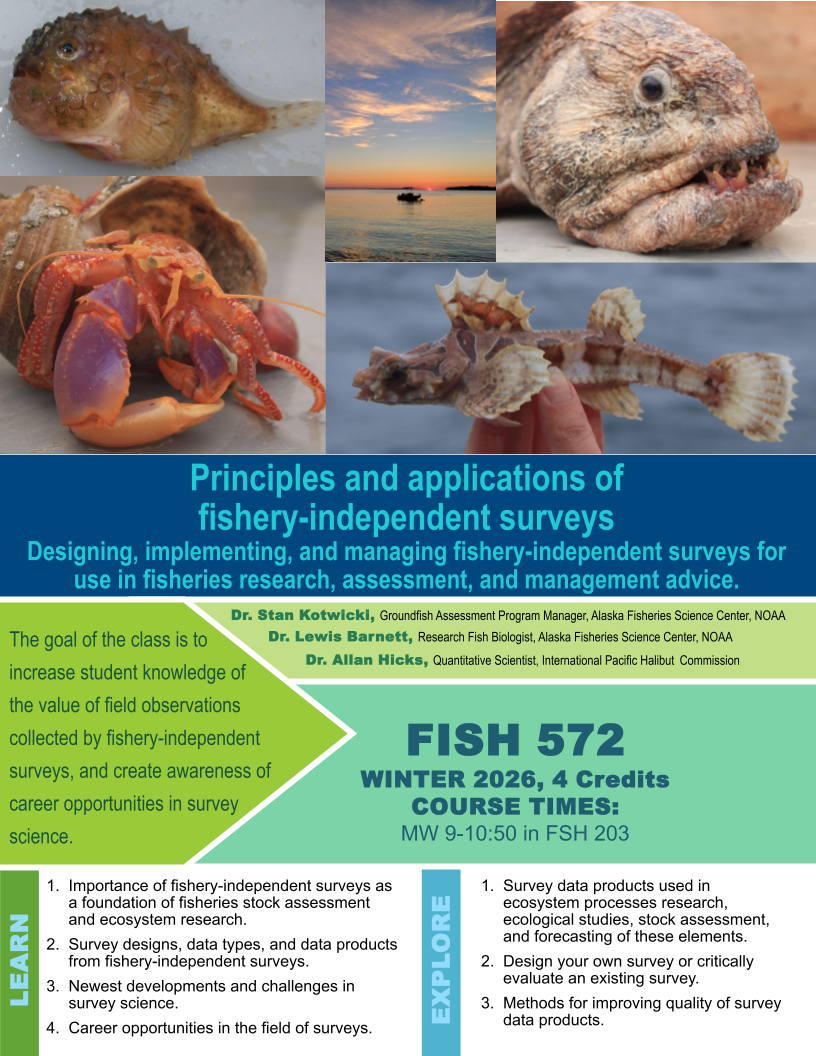
\includegraphics[keepaspectratio]{./images/FISH572-flyer.png}}

\section{Instructors}\label{instructors}

\href{https://www.fisheries.noaa.gov/contact/stan-kotwicki}{\textbf{Dr.~Stan
Kotwicki}}, Groundfish Assessment Program Manager, Alaska Fisheries
Science Center, NOAA. Stan.Kotwicki AT noaa.gov

\href{https://www.iphc.int/staff/allan-hicks-ph-d/}{\textbf{Dr.~Allan
Hicks}}, Quantitative Scientist, International Pacific Halibut
Commission. Allan.Hicks AT iphc.int

\href{https://lewisbarnett.wordpress.com/}{\textbf{Dr.~Lewis Barnett}},
Research Fish Biologist, Groundfish Assessment Program, Alaska Fisheries
Science Center, NOAA. Lewis.Barnett AT noaa.gov

\section{Class Teaching Assistants}\label{class-teaching-assistants}

\href{https://sowasser.com/}{\textbf{Dr.~Sophia Wassermann}}, Research
Fish Biologist, Alaska Fisheries Science Center, NOAA. Sophia.Wassermann
AT noaa.gov

\href{https://www.fisheries.noaa.gov/contact/emily-markowitz}{\textbf{Emily
Markowitz}}, Research Fish Biologist, Alaska Fisheries Science Center,
NOAA. Emily.Markowitz AT noaa.gov

\section{Course Summary}\label{course-summary}

The course covers the science and practice of fishery-independent
surveys, the primary monitoring approach supporting fisheries
management. Fishery-independent surveys form the foundation for stock
assessments and ecosystem research, which will be exemplified by case
studies from the field. The course covers survey designs for different
objectives, types of data collections, and data products from
fisheries-independent surveys. It explores the newest developments and
challenges in survey science, from observation to spatial and temporal
analysis, and introduces career opportunities in the field of scientific
surveys. Practical challenges in implementing these principles and
managing fisheries-independent surveys will be discussed. You will learn
how survey data products inform marine research, stock assessment,
ecosystem analysis, and ultimately accumulate into fisheries management
advice.

This course is designed for students with a background in basic
statistics, statistical modeling, and fisheries/wildlife science. It
covers a wide range of topics, including:

\begin{itemize}
\tightlist
\item
  \textbf{Survey Design}: Learn about various survey designs for
  different objectives, types of data collection, and the resulting data
  products.
\item
  \textbf{Data Analysis}: Gain practical skills in analyzing
  fisheries-independent survey data using both design- and model-based
  methods.
\item
  \textbf{Current Topics}: Explore the latest developments and
  challenges in survey science, such as uncertainty, survey continuity,
  effort optimization, flexible survey design, and the use of
  statistical tools and new technology.
\item
  \textbf{Real-World Applications}: Understand the logistical challenges
  in implementing and managing fisheries-independent surveys, and how
  survey data products are used in fisheries research, assessment, and
  management advice.
\item
  \textbf{Career Opportunities}: Discover career paths in the field of
  research surveys.
\end{itemize}

The course format includes lectures from instructors and visiting
experts, student-led literature reviews and discussions, and hands-on
survey data analysis. A significant portion of the grade is based on a
final research project using survey data, providing students with
valuable experience in research planning and execution. This class is
designed to provide useful skills for ongoing research in the field.

\bookmarksetup{startatroot}

\chapter{Course Information}\label{course-information}

\section{Lectures}\label{lectures}

Mondays and Wednesdays 9:00-10:50 am: In person in room FSH 203.

\section{Office hours}\label{office-hours}

Email instructors to set up meetings.

\section{Credits}\label{credits}

It is a 4-credit class with numerical grades. It is expected that
students will work on assignments for about 8 hours per week. Given the
limited in-class time, we expect active participation in all lectures
and discussions.

\section{Prerequisites}\label{prerequisites}

Basic statistics, statistical modeling, background in fisheries/wildlife
science; if unclear of eligibility, please correspond with the
instructor to obtain permission.

\section{Specific Learning Goals}\label{specific-learning-goals}

This class is intended to provide useful skills for your ongoing
research.

\begin{enumerate}
\def\labelenumi{\arabic{enumi}.}
\tightlist
\item
  Review types of fisheries-independent surveys and survey data products
  for ecosystem processes research, ecological studies, stock
  assessment, and forecasting within these disciplines.
\item
  Learn principles of sampling and survey designs, survey logistics and
  management, and survey data product estimation and application.
\item
  Analyze fishery-independent survey data using various statistical
  methods.
\item
  Plan research in survey science topics, e.g.~uncertainty (observation
  error), survey continuity (catchability), effort optimization,
  flexible survey design, model-based estimators, simulations,
  statistical tools, and new technology.
\item
  Complete a research project using survey data.
\item
  Learn concepts and tools for long-term strategic planning of surveys,
  including adapting monitoring programs to our changing ecosystems as
  species distributions shift due to environmental change and ecological
  interactions.
\end{enumerate}

\section{Course Material}\label{course-material}

No required text. Course materials will be selected from journals,
books, and other published scientific literature. These will be
available as PDFs through the course website. Materials will be divided
into required and optional.

\section{Course Format}\label{course-format}

\textbf{Lectures:} Lectures will take up approximately half of the
in-class time. There will be two to three lectures per week given by
instructors or visiting experts. Lectures will focus on a range of
topics, described with examples from different survey programs around
the world. Lecture slides will be made available on the course website
for downloading and reviewing.

\textbf{Literature review and discussion sections:} Students (in groups
of 1-3) will be responsible for presentations on relevant literature and
leading subsequent discussions in class. Approximately one-quarter of
in-class time will be used for these presentations and discussions.
Presentations will include a summary of relevant scientific papers on a
chosen survey-related topic, and all students will be expected to
actively participate in discussions. A list of papers for student
presentations and discussion will be provided by instructors, but
students will be given the opportunity to propose a paper of their
choice for presentations. The point of the discussion section is to read
peer-reviewed literature and become familiar with current topics in
survey science.

\textbf{Survey data analysis:} Each student will be responsible for one
mid-course project to include survey data analysis on a data set of
their choice (data sets from several actual surveys will be available,
as needed). Analysis can involve estimation of standard design-based or
model-based survey data products or could involve custom analysis for
class projects.

\textbf{Research plan and final paper:} Half of the student's grade is
based on a final written research paper using survey data. Topics for
the final paper will be proposed by students and will be presented for
class discussion and feedback within the first 3 weeks of the quarter.

\section{Grading}\label{grading}

Students will be graded on 4 tasks:

\textbf{1. Project plan - 1 page and 5 min presentation (10\% weight)}

\emph{DUE: Presentation January 14}

Within the first days of the quarter, students will be responsible for
planning a research project. Students can propose a project of their
choice as long as the data for the project are from a
fishery-independent survey. Project plans should be discussed with and
accepted by instructors. Once accepted, students will be responsible for
writing a 1-page project plan and for presenting the plan during the
class. Instructors and students will provide feedback on the plan during
the class discussion.

\textbf{2. Literature review 20-30 min presentation on the survey topic
(20\%)}

\emph{DUE: Presentation February 9}

Students will be responsible for presentations on relevant literature
and leading subsequent discussions. Literature review presentations will
be conducted on Feb 9 or later, depending on the number of
presentations. Papers for this literature review should be relevant to
the final project. Students are advised to discuss potential papers for
this review with instructors, but students will be given the opportunity
to propose a paper(s) of their choice for presentations. The literature
review presentation will be followed by a Q \& A session and in-class
discussion on the presented topics.

\textbf{3. Survey data analysis (20\%)}

\emph{DUE: 16 February}

Survey data analysis will involve estimation of standard design-based
and model-based survey data products (from provided simulated ``true
distributions'') or could involve custom analysis of survey data used
for class projects. The format of the analysis presentation will be open
and can include an analysis description with graphs and/or tables.
Analyses will be graded separately, but can be included as part of the
final paper or as an independent document. Data analysis will be due at
the end of week 6 of the course.

\textbf{4. Final project - up to 5-8 pages and 20-30 min presentation
(50\%)}

\emph{Due: Presentation March 4-11; Paper March 13}

Final project results will be presented in the form of a 20-30 minute
in-class slide presentation. Students will receive feedback from
instructors, and time for in-class discussion will be provided.
Presentations will occur during the last 2 weeks of the course. Final 5
- 8 page paper will be due at the end of week 10 and graded during the
week of finals.

\section{Grading Scale}\label{grading-scale}

Learn more about the UW
\href{https://grad.uw.edu/policies-procedures/graduate-school-memoranda/memo-19-grading-system-for-graduate-students/}{grading
scale}.

\global\setlength{\Oldarrayrulewidth}{\arrayrulewidth}

\global\setlength{\Oldtabcolsep}{\tabcolsep}

\setlength{\tabcolsep}{2pt}

\renewcommand*{\arraystretch}{1.5}



\providecommand{\ascline}[3]{\noalign{\global\arrayrulewidth #1}\arrayrulecolor[HTML]{#2}\cline{#3}}

\begin{longtable*}[c]{|p{0.75in}|p{0.75in}|p{0.75in}}



\hhline{>{\arrayrulecolor[HTML]{000000}\global\arrayrulewidth=0pt}->{\arrayrulecolor[HTML]{000000}\global\arrayrulewidth=0pt}->{\arrayrulecolor[HTML]{000000}\global\arrayrulewidth=0pt}-}

\multicolumn{1}{>{\cellcolor[HTML]{CFCFCF}\raggedright}m{\dimexpr 0.75in+0\tabcolsep}}{\textcolor[HTML]{000000}{\fontsize{11}{11}\selectfont{\global\setmainfont{Arial}{\textbf{Percent}}}}} & \multicolumn{1}{>{\cellcolor[HTML]{CFCFCF}\raggedright}m{\dimexpr 0.75in+0\tabcolsep}}{\textcolor[HTML]{000000}{\fontsize{11}{11}\selectfont{\global\setmainfont{Arial}{\textbf{GPA}}}}} & \multicolumn{1}{>{\cellcolor[HTML]{CFCFCF}\raggedright}m{\dimexpr 0.75in+0\tabcolsep}}{\textcolor[HTML]{000000}{\fontsize{11}{11}\selectfont{\global\setmainfont{Arial}{\textbf{Letter}}}}} \\

\noalign{\global\arrayrulewidth 0pt}\arrayrulecolor[HTML]{000000}

\endfirsthead 

\hhline{>{\arrayrulecolor[HTML]{000000}\global\arrayrulewidth=0pt}->{\arrayrulecolor[HTML]{000000}\global\arrayrulewidth=0pt}->{\arrayrulecolor[HTML]{000000}\global\arrayrulewidth=0pt}-}

\multicolumn{1}{>{\cellcolor[HTML]{CFCFCF}\raggedright}m{\dimexpr 0.75in+0\tabcolsep}}{\textcolor[HTML]{000000}{\fontsize{11}{11}\selectfont{\global\setmainfont{Arial}{\textbf{Percent}}}}} & \multicolumn{1}{>{\cellcolor[HTML]{CFCFCF}\raggedright}m{\dimexpr 0.75in+0\tabcolsep}}{\textcolor[HTML]{000000}{\fontsize{11}{11}\selectfont{\global\setmainfont{Arial}{\textbf{GPA}}}}} & \multicolumn{1}{>{\cellcolor[HTML]{CFCFCF}\raggedright}m{\dimexpr 0.75in+0\tabcolsep}}{\textcolor[HTML]{000000}{\fontsize{11}{11}\selectfont{\global\setmainfont{Arial}{\textbf{Letter}}}}} \\

\noalign{\global\arrayrulewidth 0pt}\arrayrulecolor[HTML]{000000}

\endhead



\multicolumn{1}{>{\cellcolor[HTML]{EFEFEF}\raggedright}m{\dimexpr 0.75in+0\tabcolsep}}{\textcolor[HTML]{000000}{\fontsize{11}{11}\selectfont{\global\setmainfont{Arial}{≥95}}}} & \multicolumn{1}{>{\cellcolor[HTML]{EFEFEF}\raggedright}m{\dimexpr 0.75in+0\tabcolsep}}{\textcolor[HTML]{000000}{\fontsize{11}{11}\selectfont{\global\setmainfont{Arial}{4}}}} & \multicolumn{1}{>{\cellcolor[HTML]{EFEFEF}\raggedright}m{\dimexpr 0.75in+0\tabcolsep}}{\textcolor[HTML]{000000}{\fontsize{11}{11}\selectfont{\global\setmainfont{Arial}{A}}}} \\

\noalign{\global\arrayrulewidth 0pt}\arrayrulecolor[HTML]{000000}





\multicolumn{1}{>{\raggedright}m{\dimexpr 0.75in+0\tabcolsep}}{\textcolor[HTML]{000000}{\fontsize{11}{11}\selectfont{\global\setmainfont{Arial}{94}}}} & \multicolumn{1}{>{\raggedright}m{\dimexpr 0.75in+0\tabcolsep}}{\textcolor[HTML]{000000}{\fontsize{11}{11}\selectfont{\global\setmainfont{Arial}{3.9}}}} & \multicolumn{1}{>{\raggedright}m{\dimexpr 0.75in+0\tabcolsep}}{\textcolor[HTML]{000000}{\fontsize{11}{11}\selectfont{\global\setmainfont{Arial}{}}}} \\

\noalign{\global\arrayrulewidth 0pt}\arrayrulecolor[HTML]{000000}





\multicolumn{1}{>{\cellcolor[HTML]{EFEFEF}\raggedright}m{\dimexpr 0.75in+0\tabcolsep}}{\textcolor[HTML]{000000}{\fontsize{11}{11}\selectfont{\global\setmainfont{Arial}{93}}}} & \multicolumn{1}{>{\cellcolor[HTML]{EFEFEF}\raggedright}m{\dimexpr 0.75in+0\tabcolsep}}{\textcolor[HTML]{000000}{\fontsize{11}{11}\selectfont{\global\setmainfont{Arial}{3.8}}}} & \multicolumn{1}{>{\cellcolor[HTML]{EFEFEF}\raggedright}m{\dimexpr 0.75in+0\tabcolsep}}{\textcolor[HTML]{000000}{\fontsize{11}{11}\selectfont{\global\setmainfont{Arial}{A-}}}} \\

\noalign{\global\arrayrulewidth 0pt}\arrayrulecolor[HTML]{000000}





\multicolumn{1}{>{\raggedright}m{\dimexpr 0.75in+0\tabcolsep}}{\textcolor[HTML]{000000}{\fontsize{11}{11}\selectfont{\global\setmainfont{Arial}{92}}}} & \multicolumn{1}{>{\raggedright}m{\dimexpr 0.75in+0\tabcolsep}}{\textcolor[HTML]{000000}{\fontsize{11}{11}\selectfont{\global\setmainfont{Arial}{3.7}}}} & \multicolumn{1}{>{\raggedright}m{\dimexpr 0.75in+0\tabcolsep}}{\textcolor[HTML]{000000}{\fontsize{11}{11}\selectfont{\global\setmainfont{Arial}{}}}} \\

\noalign{\global\arrayrulewidth 0pt}\arrayrulecolor[HTML]{000000}





\multicolumn{1}{>{\cellcolor[HTML]{EFEFEF}\raggedright}m{\dimexpr 0.75in+0\tabcolsep}}{\textcolor[HTML]{000000}{\fontsize{11}{11}\selectfont{\global\setmainfont{Arial}{91}}}} & \multicolumn{1}{>{\cellcolor[HTML]{EFEFEF}\raggedright}m{\dimexpr 0.75in+0\tabcolsep}}{\textcolor[HTML]{000000}{\fontsize{11}{11}\selectfont{\global\setmainfont{Arial}{3.6}}}} & \multicolumn{1}{>{\cellcolor[HTML]{EFEFEF}\raggedright}m{\dimexpr 0.75in+0\tabcolsep}}{\textcolor[HTML]{000000}{\fontsize{11}{11}\selectfont{\global\setmainfont{Arial}{}}}} \\

\noalign{\global\arrayrulewidth 0pt}\arrayrulecolor[HTML]{000000}





\multicolumn{1}{>{\raggedright}m{\dimexpr 0.75in+0\tabcolsep}}{\textcolor[HTML]{000000}{\fontsize{11}{11}\selectfont{\global\setmainfont{Arial}{90}}}} & \multicolumn{1}{>{\raggedright}m{\dimexpr 0.75in+0\tabcolsep}}{\textcolor[HTML]{000000}{\fontsize{11}{11}\selectfont{\global\setmainfont{Arial}{3.5}}}} & \multicolumn{1}{>{\raggedright}m{\dimexpr 0.75in+0\tabcolsep}}{\textcolor[HTML]{000000}{\fontsize{11}{11}\selectfont{\global\setmainfont{Arial}{}}}} \\

\noalign{\global\arrayrulewidth 0pt}\arrayrulecolor[HTML]{000000}





\multicolumn{1}{>{\cellcolor[HTML]{EFEFEF}\raggedright}m{\dimexpr 0.75in+0\tabcolsep}}{\textcolor[HTML]{000000}{\fontsize{11}{11}\selectfont{\global\setmainfont{Arial}{89}}}} & \multicolumn{1}{>{\cellcolor[HTML]{EFEFEF}\raggedright}m{\dimexpr 0.75in+0\tabcolsep}}{\textcolor[HTML]{000000}{\fontsize{11}{11}\selectfont{\global\setmainfont{Arial}{3.4}}}} & \multicolumn{1}{>{\cellcolor[HTML]{EFEFEF}\raggedright}m{\dimexpr 0.75in+0\tabcolsep}}{\textcolor[HTML]{000000}{\fontsize{11}{11}\selectfont{\global\setmainfont{Arial}{B+}}}} \\

\noalign{\global\arrayrulewidth 0pt}\arrayrulecolor[HTML]{000000}





\multicolumn{1}{>{\raggedright}m{\dimexpr 0.75in+0\tabcolsep}}{\textcolor[HTML]{000000}{\fontsize{11}{11}\selectfont{\global\setmainfont{Arial}{88}}}} & \multicolumn{1}{>{\raggedright}m{\dimexpr 0.75in+0\tabcolsep}}{\textcolor[HTML]{000000}{\fontsize{11}{11}\selectfont{\global\setmainfont{Arial}{3.3}}}} & \multicolumn{1}{>{\raggedright}m{\dimexpr 0.75in+0\tabcolsep}}{\textcolor[HTML]{000000}{\fontsize{11}{11}\selectfont{\global\setmainfont{Arial}{}}}} \\

\noalign{\global\arrayrulewidth 0pt}\arrayrulecolor[HTML]{000000}





\multicolumn{1}{>{\cellcolor[HTML]{EFEFEF}\raggedright}m{\dimexpr 0.75in+0\tabcolsep}}{\textcolor[HTML]{000000}{\fontsize{11}{11}\selectfont{\global\setmainfont{Arial}{87}}}} & \multicolumn{1}{>{\cellcolor[HTML]{EFEFEF}\raggedright}m{\dimexpr 0.75in+0\tabcolsep}}{\textcolor[HTML]{000000}{\fontsize{11}{11}\selectfont{\global\setmainfont{Arial}{3.2}}}} & \multicolumn{1}{>{\cellcolor[HTML]{EFEFEF}\raggedright}m{\dimexpr 0.75in+0\tabcolsep}}{\textcolor[HTML]{000000}{\fontsize{11}{11}\selectfont{\global\setmainfont{Arial}{}}}} \\

\noalign{\global\arrayrulewidth 0pt}\arrayrulecolor[HTML]{000000}





\multicolumn{1}{>{\raggedright}m{\dimexpr 0.75in+0\tabcolsep}}{\textcolor[HTML]{000000}{\fontsize{11}{11}\selectfont{\global\setmainfont{Arial}{86}}}} & \multicolumn{1}{>{\raggedright}m{\dimexpr 0.75in+0\tabcolsep}}{\textcolor[HTML]{000000}{\fontsize{11}{11}\selectfont{\global\setmainfont{Arial}{3.1}}}} & \multicolumn{1}{>{\raggedright}m{\dimexpr 0.75in+0\tabcolsep}}{\textcolor[HTML]{000000}{\fontsize{11}{11}\selectfont{\global\setmainfont{Arial}{}}}} \\

\noalign{\global\arrayrulewidth 0pt}\arrayrulecolor[HTML]{000000}





\multicolumn{1}{>{\cellcolor[HTML]{EFEFEF}\raggedright}m{\dimexpr 0.75in+0\tabcolsep}}{\textcolor[HTML]{000000}{\fontsize{11}{11}\selectfont{\global\setmainfont{Arial}{85}}}} & \multicolumn{1}{>{\cellcolor[HTML]{EFEFEF}\raggedright}m{\dimexpr 0.75in+0\tabcolsep}}{\textcolor[HTML]{000000}{\fontsize{11}{11}\selectfont{\global\setmainfont{Arial}{3}}}} & \multicolumn{1}{>{\cellcolor[HTML]{EFEFEF}\raggedright}m{\dimexpr 0.75in+0\tabcolsep}}{\textcolor[HTML]{000000}{\fontsize{11}{11}\selectfont{\global\setmainfont{Arial}{B}}}} \\

\noalign{\global\arrayrulewidth 0pt}\arrayrulecolor[HTML]{000000}





\multicolumn{1}{>{\raggedright}m{\dimexpr 0.75in+0\tabcolsep}}{\textcolor[HTML]{000000}{\fontsize{11}{11}\selectfont{\global\setmainfont{Arial}{84}}}} & \multicolumn{1}{>{\raggedright}m{\dimexpr 0.75in+0\tabcolsep}}{\textcolor[HTML]{000000}{\fontsize{11}{11}\selectfont{\global\setmainfont{Arial}{2.9}}}} & \multicolumn{1}{>{\raggedright}m{\dimexpr 0.75in+0\tabcolsep}}{\textcolor[HTML]{000000}{\fontsize{11}{11}\selectfont{\global\setmainfont{Arial}{}}}} \\

\noalign{\global\arrayrulewidth 0pt}\arrayrulecolor[HTML]{000000}





\multicolumn{1}{>{\cellcolor[HTML]{EFEFEF}\raggedright}m{\dimexpr 0.75in+0\tabcolsep}}{\textcolor[HTML]{000000}{\fontsize{11}{11}\selectfont{\global\setmainfont{Arial}{83}}}} & \multicolumn{1}{>{\cellcolor[HTML]{EFEFEF}\raggedright}m{\dimexpr 0.75in+0\tabcolsep}}{\textcolor[HTML]{000000}{\fontsize{11}{11}\selectfont{\global\setmainfont{Arial}{2.8}}}} & \multicolumn{1}{>{\cellcolor[HTML]{EFEFEF}\raggedright}m{\dimexpr 0.75in+0\tabcolsep}}{\textcolor[HTML]{000000}{\fontsize{11}{11}\selectfont{\global\setmainfont{Arial}{B-}}}} \\

\noalign{\global\arrayrulewidth 0pt}\arrayrulecolor[HTML]{000000}





\multicolumn{1}{>{\raggedright}m{\dimexpr 0.75in+0\tabcolsep}}{\textcolor[HTML]{000000}{\fontsize{11}{11}\selectfont{\global\setmainfont{Arial}{82}}}} & \multicolumn{1}{>{\raggedright}m{\dimexpr 0.75in+0\tabcolsep}}{\textcolor[HTML]{000000}{\fontsize{11}{11}\selectfont{\global\setmainfont{Arial}{2.7}}}} & \multicolumn{1}{>{\raggedright}m{\dimexpr 0.75in+0\tabcolsep}}{\textcolor[HTML]{000000}{\fontsize{11}{11}\selectfont{\global\setmainfont{Arial}{B-}}}} \\

\noalign{\global\arrayrulewidth 0pt}\arrayrulecolor[HTML]{000000}





\multicolumn{1}{>{\cellcolor[HTML]{EFEFEF}\raggedright}m{\dimexpr 0.75in+0\tabcolsep}}{\textcolor[HTML]{000000}{\fontsize{11}{11}\selectfont{\global\setmainfont{Arial}{81}}}} & \multicolumn{1}{>{\cellcolor[HTML]{EFEFEF}\raggedright}m{\dimexpr 0.75in+0\tabcolsep}}{\textcolor[HTML]{000000}{\fontsize{11}{11}\selectfont{\global\setmainfont{Arial}{2.6}}}} & \multicolumn{1}{>{\cellcolor[HTML]{EFEFEF}\raggedright}m{\dimexpr 0.75in+0\tabcolsep}}{\textcolor[HTML]{000000}{\fontsize{11}{11}\selectfont{\global\setmainfont{Arial}{}}}} \\

\noalign{\global\arrayrulewidth 0pt}\arrayrulecolor[HTML]{000000}





\multicolumn{1}{>{\raggedright}m{\dimexpr 0.75in+0\tabcolsep}}{\textcolor[HTML]{000000}{\fontsize{11}{11}\selectfont{\global\setmainfont{Arial}{80}}}} & \multicolumn{1}{>{\raggedright}m{\dimexpr 0.75in+0\tabcolsep}}{\textcolor[HTML]{000000}{\fontsize{11}{11}\selectfont{\global\setmainfont{Arial}{2.5}}}} & \multicolumn{1}{>{\raggedright}m{\dimexpr 0.75in+0\tabcolsep}}{\textcolor[HTML]{000000}{\fontsize{11}{11}\selectfont{\global\setmainfont{Arial}{}}}} \\

\noalign{\global\arrayrulewidth 0pt}\arrayrulecolor[HTML]{000000}





\multicolumn{1}{>{\cellcolor[HTML]{EFEFEF}\raggedright}m{\dimexpr 0.75in+0\tabcolsep}}{\textcolor[HTML]{000000}{\fontsize{11}{11}\selectfont{\global\setmainfont{Arial}{79}}}} & \multicolumn{1}{>{\cellcolor[HTML]{EFEFEF}\raggedright}m{\dimexpr 0.75in+0\tabcolsep}}{\textcolor[HTML]{000000}{\fontsize{11}{11}\selectfont{\global\setmainfont{Arial}{2.4}}}} & \multicolumn{1}{>{\cellcolor[HTML]{EFEFEF}\raggedright}m{\dimexpr 0.75in+0\tabcolsep}}{\textcolor[HTML]{000000}{\fontsize{11}{11}\selectfont{\global\setmainfont{Arial}{C+}}}} \\

\noalign{\global\arrayrulewidth 0pt}\arrayrulecolor[HTML]{000000}





\multicolumn{1}{>{\raggedright}m{\dimexpr 0.75in+0\tabcolsep}}{\textcolor[HTML]{000000}{\fontsize{11}{11}\selectfont{\global\setmainfont{Arial}{78}}}} & \multicolumn{1}{>{\raggedright}m{\dimexpr 0.75in+0\tabcolsep}}{\textcolor[HTML]{000000}{\fontsize{11}{11}\selectfont{\global\setmainfont{Arial}{2.3}}}} & \multicolumn{1}{>{\raggedright}m{\dimexpr 0.75in+0\tabcolsep}}{\textcolor[HTML]{000000}{\fontsize{11}{11}\selectfont{\global\setmainfont{Arial}{}}}} \\

\noalign{\global\arrayrulewidth 0pt}\arrayrulecolor[HTML]{000000}





\multicolumn{1}{>{\cellcolor[HTML]{EFEFEF}\raggedright}m{\dimexpr 0.75in+0\tabcolsep}}{\textcolor[HTML]{000000}{\fontsize{11}{11}\selectfont{\global\setmainfont{Arial}{77}}}} & \multicolumn{1}{>{\cellcolor[HTML]{EFEFEF}\raggedright}m{\dimexpr 0.75in+0\tabcolsep}}{\textcolor[HTML]{000000}{\fontsize{11}{11}\selectfont{\global\setmainfont{Arial}{2.2}}}} & \multicolumn{1}{>{\cellcolor[HTML]{EFEFEF}\raggedright}m{\dimexpr 0.75in+0\tabcolsep}}{\textcolor[HTML]{000000}{\fontsize{11}{11}\selectfont{\global\setmainfont{Arial}{}}}} \\

\noalign{\global\arrayrulewidth 0pt}\arrayrulecolor[HTML]{000000}





\multicolumn{1}{>{\raggedright}m{\dimexpr 0.75in+0\tabcolsep}}{\textcolor[HTML]{000000}{\fontsize{11}{11}\selectfont{\global\setmainfont{Arial}{76}}}} & \multicolumn{1}{>{\raggedright}m{\dimexpr 0.75in+0\tabcolsep}}{\textcolor[HTML]{000000}{\fontsize{11}{11}\selectfont{\global\setmainfont{Arial}{2.1}}}} & \multicolumn{1}{>{\raggedright}m{\dimexpr 0.75in+0\tabcolsep}}{\textcolor[HTML]{000000}{\fontsize{11}{11}\selectfont{\global\setmainfont{Arial}{}}}} \\

\noalign{\global\arrayrulewidth 0pt}\arrayrulecolor[HTML]{000000}





\multicolumn{1}{>{\cellcolor[HTML]{EFEFEF}\raggedright}m{\dimexpr 0.75in+0\tabcolsep}}{\textcolor[HTML]{000000}{\fontsize{11}{11}\selectfont{\global\setmainfont{Arial}{75}}}} & \multicolumn{1}{>{\cellcolor[HTML]{EFEFEF}\raggedright}m{\dimexpr 0.75in+0\tabcolsep}}{\textcolor[HTML]{000000}{\fontsize{11}{11}\selectfont{\global\setmainfont{Arial}{2}}}} & \multicolumn{1}{>{\cellcolor[HTML]{EFEFEF}\raggedright}m{\dimexpr 0.75in+0\tabcolsep}}{\textcolor[HTML]{000000}{\fontsize{11}{11}\selectfont{\global\setmainfont{Arial}{C}}}} \\

\noalign{\global\arrayrulewidth 0pt}\arrayrulecolor[HTML]{000000}





\multicolumn{1}{>{\raggedright}m{\dimexpr 0.75in+0\tabcolsep}}{\textcolor[HTML]{000000}{\fontsize{11}{11}\selectfont{\global\setmainfont{Arial}{74}}}} & \multicolumn{1}{>{\raggedright}m{\dimexpr 0.75in+0\tabcolsep}}{\textcolor[HTML]{000000}{\fontsize{11}{11}\selectfont{\global\setmainfont{Arial}{1.9}}}} & \multicolumn{1}{>{\raggedright}m{\dimexpr 0.75in+0\tabcolsep}}{\textcolor[HTML]{000000}{\fontsize{11}{11}\selectfont{\global\setmainfont{Arial}{}}}} \\

\noalign{\global\arrayrulewidth 0pt}\arrayrulecolor[HTML]{000000}





\multicolumn{1}{>{\cellcolor[HTML]{EFEFEF}\raggedright}m{\dimexpr 0.75in+0\tabcolsep}}{\textcolor[HTML]{000000}{\fontsize{11}{11}\selectfont{\global\setmainfont{Arial}{73}}}} & \multicolumn{1}{>{\cellcolor[HTML]{EFEFEF}\raggedright}m{\dimexpr 0.75in+0\tabcolsep}}{\textcolor[HTML]{000000}{\fontsize{11}{11}\selectfont{\global\setmainfont{Arial}{1.8}}}} & \multicolumn{1}{>{\cellcolor[HTML]{EFEFEF}\raggedright}m{\dimexpr 0.75in+0\tabcolsep}}{\textcolor[HTML]{000000}{\fontsize{11}{11}\selectfont{\global\setmainfont{Arial}{}}}} \\

\noalign{\global\arrayrulewidth 0pt}\arrayrulecolor[HTML]{000000}





\multicolumn{1}{>{\raggedright}m{\dimexpr 0.75in+0\tabcolsep}}{\textcolor[HTML]{000000}{\fontsize{11}{11}\selectfont{\global\setmainfont{Arial}{72}}}} & \multicolumn{1}{>{\raggedright}m{\dimexpr 0.75in+0\tabcolsep}}{\textcolor[HTML]{000000}{\fontsize{11}{11}\selectfont{\global\setmainfont{Arial}{1.7}}}} & \multicolumn{1}{>{\raggedright}m{\dimexpr 0.75in+0\tabcolsep}}{\textcolor[HTML]{000000}{\fontsize{11}{11}\selectfont{\global\setmainfont{Arial}{}}}} \\

\noalign{\global\arrayrulewidth 0pt}\arrayrulecolor[HTML]{000000}





\multicolumn{1}{>{\cellcolor[HTML]{EFEFEF}\raggedright}m{\dimexpr 0.75in+0\tabcolsep}}{\textcolor[HTML]{000000}{\fontsize{11}{11}\selectfont{\global\setmainfont{Arial}{<72}}}} & \multicolumn{1}{>{\cellcolor[HTML]{EFEFEF}\raggedright}m{\dimexpr 0.75in+0\tabcolsep}}{\textcolor[HTML]{000000}{\fontsize{11}{11}\selectfont{\global\setmainfont{Arial}{1.6-\ 0.0}}}} & \multicolumn{1}{>{\cellcolor[HTML]{EFEFEF}\raggedright}m{\dimexpr 0.75in+0\tabcolsep}}{\textcolor[HTML]{000000}{\fontsize{11}{11}\selectfont{\global\setmainfont{Arial}{E}}}} \\

\noalign{\global\arrayrulewidth 0pt}\arrayrulecolor[HTML]{000000}





\end{longtable*}



\arrayrulecolor[HTML]{000000}

\global\setlength{\arrayrulewidth}{\Oldarrayrulewidth}

\global\setlength{\tabcolsep}{\Oldtabcolsep}

\renewcommand*{\arraystretch}{1}

\section{Lecture plan}\label{lecture-plan}

\href{https://uw.iasystem.org/survey/268860}{Please fill out a class
evaluation!}

\global\setlength{\Oldarrayrulewidth}{\arrayrulewidth}

\global\setlength{\Oldtabcolsep}{\tabcolsep}

\setlength{\tabcolsep}{2pt}

\renewcommand*{\arraystretch}{1.5}



\providecommand{\ascline}[3]{\noalign{\global\arrayrulewidth #1}\arrayrulecolor[HTML]{#2}\cline{#3}}

\begin{longtable*}[c]{|p{0.75in}|p{0.75in}|p{0.75in}|p{0.75in}|p{4.00in}}



\hhline{>{\arrayrulecolor[HTML]{000000}\global\arrayrulewidth=0pt}->{\arrayrulecolor[HTML]{000000}\global\arrayrulewidth=0pt}->{\arrayrulecolor[HTML]{000000}\global\arrayrulewidth=0pt}->{\arrayrulecolor[HTML]{000000}\global\arrayrulewidth=0pt}->{\arrayrulecolor[HTML]{000000}\global\arrayrulewidth=0pt}-}

\multicolumn{1}{>{\cellcolor[HTML]{CFCFCF}\raggedleft}m{\dimexpr 0.75in+0\tabcolsep}}{\textcolor[HTML]{000000}{\fontsize{11}{11}\selectfont{\global\setmainfont{Arial}{\textbf{Week}}}}} & \multicolumn{1}{>{\cellcolor[HTML]{CFCFCF}\raggedright}m{\dimexpr 0.75in+0\tabcolsep}}{\textcolor[HTML]{000000}{\fontsize{11}{11}\selectfont{\global\setmainfont{Arial}{\textbf{Date}}}}} & \multicolumn{1}{>{\cellcolor[HTML]{CFCFCF}\raggedleft}m{\dimexpr 0.75in+0\tabcolsep}}{\textcolor[HTML]{000000}{\fontsize{11}{11}\selectfont{\global\setmainfont{Arial}{\textbf{Lecture}}}}} & \multicolumn{1}{>{\cellcolor[HTML]{CFCFCF}\raggedright}m{\dimexpr 0.75in+0\tabcolsep}}{\textcolor[HTML]{000000}{\fontsize{11}{11}\selectfont{\global\setmainfont{Arial}{\textbf{Instructor}}}}} & \multicolumn{1}{>{\cellcolor[HTML]{CFCFCF}\raggedright}m{\dimexpr 4in+0\tabcolsep}}{\textcolor[HTML]{000000}{\fontsize{11}{11}\selectfont{\global\setmainfont{Arial}{\textbf{Description}}}}} \\

\noalign{\global\arrayrulewidth 0pt}\arrayrulecolor[HTML]{000000}

\endfirsthead 

\hhline{>{\arrayrulecolor[HTML]{000000}\global\arrayrulewidth=0pt}->{\arrayrulecolor[HTML]{000000}\global\arrayrulewidth=0pt}->{\arrayrulecolor[HTML]{000000}\global\arrayrulewidth=0pt}->{\arrayrulecolor[HTML]{000000}\global\arrayrulewidth=0pt}->{\arrayrulecolor[HTML]{000000}\global\arrayrulewidth=0pt}-}

\multicolumn{1}{>{\cellcolor[HTML]{CFCFCF}\raggedleft}m{\dimexpr 0.75in+0\tabcolsep}}{\textcolor[HTML]{000000}{\fontsize{11}{11}\selectfont{\global\setmainfont{Arial}{\textbf{Week}}}}} & \multicolumn{1}{>{\cellcolor[HTML]{CFCFCF}\raggedright}m{\dimexpr 0.75in+0\tabcolsep}}{\textcolor[HTML]{000000}{\fontsize{11}{11}\selectfont{\global\setmainfont{Arial}{\textbf{Date}}}}} & \multicolumn{1}{>{\cellcolor[HTML]{CFCFCF}\raggedleft}m{\dimexpr 0.75in+0\tabcolsep}}{\textcolor[HTML]{000000}{\fontsize{11}{11}\selectfont{\global\setmainfont{Arial}{\textbf{Lecture}}}}} & \multicolumn{1}{>{\cellcolor[HTML]{CFCFCF}\raggedright}m{\dimexpr 0.75in+0\tabcolsep}}{\textcolor[HTML]{000000}{\fontsize{11}{11}\selectfont{\global\setmainfont{Arial}{\textbf{Instructor}}}}} & \multicolumn{1}{>{\cellcolor[HTML]{CFCFCF}\raggedright}m{\dimexpr 4in+0\tabcolsep}}{\textcolor[HTML]{000000}{\fontsize{11}{11}\selectfont{\global\setmainfont{Arial}{\textbf{Description}}}}} \\

\noalign{\global\arrayrulewidth 0pt}\arrayrulecolor[HTML]{000000}

\endhead



\multicolumn{1}{>{\cellcolor[HTML]{D3D3D3}\raggedleft}m{\dimexpr 0.75in+0\tabcolsep}}{} & \multicolumn{1}{>{\cellcolor[HTML]{EFEFEF}\raggedright}m{\dimexpr 0.75in+0\tabcolsep}}{\textcolor[HTML]{000000}{\fontsize{11}{11}\selectfont{\global\setmainfont{Arial}{Jan\ 5}}}} & \multicolumn{1}{>{\cellcolor[HTML]{EFEFEF}\raggedleft}m{\dimexpr 0.75in+0\tabcolsep}}{\textcolor[HTML]{000000}{\fontsize{11}{11}\selectfont{\global\setmainfont{Arial}{1}}}} & \multicolumn{1}{>{\cellcolor[HTML]{EFEFEF}\raggedright}m{\dimexpr 0.75in+0\tabcolsep}}{\textcolor[HTML]{000000}{\fontsize{11}{11}\selectfont{\global\setmainfont{Arial}{Kotwicki\ (Wassermann)}}}} & \multicolumn{1}{>{\cellcolor[HTML]{EFEFEF}\raggedright}m{\dimexpr 4in+0\tabcolsep}}{\textcolor[HTML]{000000}{\fontsize{11}{11}\selectfont{\global\setmainfont{Arial}{Course\ outline\ and\ introductions.\ Overview\ of\ fisheries\ dependent\ and\ independent\ data\ collection,\ types\ of\ fisheries\ surveys,\ and\ other\ survey\ science\ topics.\ Describe\ potential\ class\ project.\ Provide\ examples.}}}\textcolor[HTML]{000000}{\fontsize{11}{11}\selectfont{\global\setmainfont{Arial}{\linebreak }}}\textcolor[HTML]{000000}{\fontsize{11}{11}\selectfont{\global\setmainfont{Arial}{Guest\ Lectures:\ Lyle\ Britt\ (AFSC),\ Denise\ McKelvey\ (AFSC)}}}} \\

\noalign{\global\arrayrulewidth 0pt}\arrayrulecolor[HTML]{000000}

\hhline{>{\arrayrulecolor[HTML]{666666}\global\arrayrulewidth=1pt}->{\arrayrulecolor[HTML]{666666}\global\arrayrulewidth=1pt}->{\arrayrulecolor[HTML]{666666}\global\arrayrulewidth=1pt}->{\arrayrulecolor[HTML]{666666}\global\arrayrulewidth=1pt}->{\arrayrulecolor[HTML]{666666}\global\arrayrulewidth=1pt}-}



\multicolumn{1}{>{\cellcolor[HTML]{D3D3D3}\raggedleft}m{\dimexpr 0.75in+0\tabcolsep}}{\multirow[c]{-2}{*}{\parbox{0.75in}{\raggedleft \textcolor[HTML]{000000}{\fontsize{11}{11}\selectfont{\global\setmainfont{Arial}{1}}}}}} & \multicolumn{1}{>{\raggedright}m{\dimexpr 0.75in+0\tabcolsep}}{\textcolor[HTML]{000000}{\fontsize{11}{11}\selectfont{\global\setmainfont{Arial}{Jan\ 7}}}} & \multicolumn{1}{>{\raggedleft}m{\dimexpr 0.75in+0\tabcolsep}}{\textcolor[HTML]{000000}{\fontsize{11}{11}\selectfont{\global\setmainfont{Arial}{2}}}} & \multicolumn{1}{>{\raggedright}m{\dimexpr 0.75in+0\tabcolsep}}{\textcolor[HTML]{000000}{\fontsize{11}{11}\selectfont{\global\setmainfont{Arial}{Kotwicki\ (Markowitz)}}}} & \multicolumn{1}{>{\raggedright}m{\dimexpr 4in+0\tabcolsep}}{\textcolor[HTML]{000000}{\fontsize{11}{11}\selectfont{\global\setmainfont{Arial}{Overview\ of\ survey\ data\ products\ for\ ecosystem\ processes\ research,\ ecological\ studies,\ stock\ assessment,\ and\ forecasting.\ }}}\textcolor[HTML]{000000}{\fontsize{11}{11}\selectfont{\global\setmainfont{Arial}{\linebreak }}}\textcolor[HTML]{000000}{\fontsize{11}{11}\selectfont{\global\setmainfont{Arial}{Guest\ Lectures:\ Kayla\ Ualesi\ (IPHC),\ Ebett\ Siddon\ (NOAA)}}}} \\

\noalign{\global\arrayrulewidth 0pt}\arrayrulecolor[HTML]{000000}

\hhline{>{\arrayrulecolor[HTML]{666666}\global\arrayrulewidth=1pt}->{\arrayrulecolor[HTML]{666666}\global\arrayrulewidth=1pt}->{\arrayrulecolor[HTML]{666666}\global\arrayrulewidth=1pt}->{\arrayrulecolor[HTML]{666666}\global\arrayrulewidth=1pt}->{\arrayrulecolor[HTML]{666666}\global\arrayrulewidth=1pt}-}



\multicolumn{1}{>{\cellcolor[HTML]{BEBEBE}\raggedleft}m{\dimexpr 0.75in+0\tabcolsep}}{} & \multicolumn{1}{>{\cellcolor[HTML]{EFEFEF}\raggedright}m{\dimexpr 0.75in+0\tabcolsep}}{\textcolor[HTML]{000000}{\fontsize{11}{11}\selectfont{\global\setmainfont{Arial}{Jan\ 12}}}} & \multicolumn{1}{>{\cellcolor[HTML]{EFEFEF}\raggedleft}m{\dimexpr 0.75in+0\tabcolsep}}{\textcolor[HTML]{000000}{\fontsize{11}{11}\selectfont{\global\setmainfont{Arial}{3}}}} & \multicolumn{1}{>{\cellcolor[HTML]{EFEFEF}\raggedright}m{\dimexpr 0.75in+0\tabcolsep}}{\textcolor[HTML]{000000}{\fontsize{11}{11}\selectfont{\global\setmainfont{Arial}{Hicks\ (Markowitz)}}}} & \multicolumn{1}{>{\cellcolor[HTML]{EFEFEF}\raggedright}m{\dimexpr 4in+0\tabcolsep}}{\textcolor[HTML]{000000}{\fontsize{11}{11}\selectfont{\global\setmainfont{Arial}{Guest\ presentation.\ Design\ principles,\ sampling\ designs,\ logistics\ and\ estimation.\ (Ray\ Webster)\ }}}\textcolor[HTML]{000000}{\fontsize{11}{11}\selectfont{\global\setmainfont{Arial}{\linebreak }}}\textcolor[HTML]{000000}{\fontsize{11}{11}\selectfont{\global\setmainfont{Arial}{Guest\ presentation.\ Case\ study\ for\ implementing\ survey\ design\ (Zack\ Oyafuso).}}}} \\

\noalign{\global\arrayrulewidth 0pt}\arrayrulecolor[HTML]{000000}

\hhline{>{\arrayrulecolor[HTML]{666666}\global\arrayrulewidth=1pt}->{\arrayrulecolor[HTML]{666666}\global\arrayrulewidth=1pt}->{\arrayrulecolor[HTML]{666666}\global\arrayrulewidth=1pt}->{\arrayrulecolor[HTML]{666666}\global\arrayrulewidth=1pt}->{\arrayrulecolor[HTML]{666666}\global\arrayrulewidth=1pt}-}



\multicolumn{1}{>{\cellcolor[HTML]{BEBEBE}\raggedleft}m{\dimexpr 0.75in+0\tabcolsep}}{\multirow[c]{-2}{*}{\parbox{0.75in}{\raggedleft \textcolor[HTML]{000000}{\fontsize{11}{11}\selectfont{\global\setmainfont{Arial}{2}}}}}} & \multicolumn{1}{>{\raggedright}m{\dimexpr 0.75in+0\tabcolsep}}{\textcolor[HTML]{000000}{\fontsize{11}{11}\selectfont{\global\setmainfont{Arial}{Jan\ 14}}}} & \multicolumn{1}{>{\raggedleft}m{\dimexpr 0.75in+0\tabcolsep}}{\textcolor[HTML]{000000}{\fontsize{11}{11}\selectfont{\global\setmainfont{Arial}{4}}}} & \multicolumn{1}{>{\raggedright}m{\dimexpr 0.75in+0\tabcolsep}}{\textcolor[HTML]{000000}{\fontsize{11}{11}\selectfont{\global\setmainfont{Arial}{Kotwicki\ (Markowitz)}}}} & \multicolumn{1}{>{\raggedright}m{\dimexpr 4in+0\tabcolsep}}{\textcolor[HTML]{000000}{\fontsize{11}{11}\selectfont{\global\setmainfont{Arial}{Student\ presentations\ on\ project\ plan:\ 5\ minutes\ presentation,\ 5-10\ minutes\ for\ discussion.}}}\textcolor[HTML]{000000}{\fontsize{11}{11}\selectfont{\global\setmainfont{Arial}{\linebreak }}}\textcolor[HTML]{000000}{\fontsize{11}{11}\selectfont{\global\setmainfont{Arial}{Some\ general\ topics}}}\textcolor[HTML]{000000}{\fontsize{11}{11}\selectfont{\global\setmainfont{Arial}{\linebreak }}}\textcolor[HTML]{000000}{\fontsize{11}{11}\selectfont{\global\setmainfont{Arial}{a.\ Design\ of\ a\ new\ survey\ from\ the\ ground\ up.}}}\textcolor[HTML]{000000}{\fontsize{11}{11}\selectfont{\global\setmainfont{Arial}{\linebreak }}}\textcolor[HTML]{000000}{\fontsize{11}{11}\selectfont{\global\setmainfont{Arial}{b.\ Analysis\ of\ existing\ survey\ data\ (e.g.\ present\ survey\ data\ product\ and\ its\ uncertainty,\ use\ of\ survey\ data\ in\ assessments,\ role\ of\ uncertainty\ in\ assessment).}}}\textcolor[HTML]{000000}{\fontsize{11}{11}\selectfont{\global\setmainfont{Arial}{\linebreak }}}\textcolor[HTML]{000000}{\fontsize{11}{11}\selectfont{\global\setmainfont{Arial}{c.\ Literature\ review\ of\ a\ survey\ topic\ under\ active\ research.}}}\textcolor[HTML]{000000}{\fontsize{11}{11}\selectfont{\global\setmainfont{Arial}{\linebreak }}}\textcolor[HTML]{000000}{\fontsize{11}{11}\selectfont{\global\setmainfont{Arial}{\linebreak }}}\textcolor[HTML]{000000}{\fontsize{11}{11}\selectfont{\global\setmainfont{Arial}{Examples\ of\ literature\ overview.\ Opportunity\ for\ students\ to\ ask\ questions\ about\ class\ projects.}}}} \\

\noalign{\global\arrayrulewidth 0pt}\arrayrulecolor[HTML]{000000}

\hhline{>{\arrayrulecolor[HTML]{666666}\global\arrayrulewidth=1pt}->{\arrayrulecolor[HTML]{666666}\global\arrayrulewidth=1pt}->{\arrayrulecolor[HTML]{666666}\global\arrayrulewidth=1pt}->{\arrayrulecolor[HTML]{666666}\global\arrayrulewidth=1pt}->{\arrayrulecolor[HTML]{666666}\global\arrayrulewidth=1pt}-}



\multicolumn{1}{>{\cellcolor[HTML]{D3D3D3}\raggedleft}m{\dimexpr 0.75in+0\tabcolsep}}{} & \multicolumn{1}{>{\cellcolor[HTML]{EFEFEF}\raggedright}m{\dimexpr 0.75in+0\tabcolsep}}{\textcolor[HTML]{000000}{\fontsize{11}{11}\selectfont{\global\setmainfont{Arial}{Jan\ 19}}}} & \multicolumn{1}{>{\cellcolor[HTML]{EFEFEF}\raggedleft}m{\dimexpr 0.75in+0\tabcolsep}}{\textcolor[HTML]{000000}{\fontsize{11}{11}\selectfont{\global\setmainfont{Arial}{}}}} & \multicolumn{2}{>{\cellcolor[HTML]{EFEFEF}\raggedright}m{\dimexpr 4.75in+2\tabcolsep}}{\textcolor[HTML]{000000}{\fontsize{11}{11}\selectfont{\global\setmainfont{Arial}{\textit{Martin\ Luther\ King\ Jr.\ Observed\ Holiday}}}}} \\

\noalign{\global\arrayrulewidth 0pt}\arrayrulecolor[HTML]{000000}

\hhline{>{\arrayrulecolor[HTML]{666666}\global\arrayrulewidth=1pt}->{\arrayrulecolor[HTML]{666666}\global\arrayrulewidth=1pt}->{\arrayrulecolor[HTML]{666666}\global\arrayrulewidth=1pt}->{\arrayrulecolor[HTML]{666666}\global\arrayrulewidth=1pt}->{\arrayrulecolor[HTML]{666666}\global\arrayrulewidth=1pt}-}



\multicolumn{1}{>{\cellcolor[HTML]{D3D3D3}\raggedleft}m{\dimexpr 0.75in+0\tabcolsep}}{\multirow[c]{-2}{*}{\parbox{0.75in}{\raggedleft \textcolor[HTML]{000000}{\fontsize{11}{11}\selectfont{\global\setmainfont{Arial}{3}}}}}} & \multicolumn{1}{>{\raggedright}m{\dimexpr 0.75in+0\tabcolsep}}{\textcolor[HTML]{000000}{\fontsize{11}{11}\selectfont{\global\setmainfont{Arial}{Jan\ 21}}}} & \multicolumn{1}{>{\raggedleft}m{\dimexpr 0.75in+0\tabcolsep}}{\textcolor[HTML]{000000}{\fontsize{11}{11}\selectfont{\global\setmainfont{Arial}{5}}}} & \multicolumn{1}{>{\raggedright}m{\dimexpr 0.75in+0\tabcolsep}}{\textcolor[HTML]{000000}{\fontsize{11}{11}\selectfont{\global\setmainfont{Arial}{Kotwicki\ (Wassermann)}}}} & \multicolumn{1}{>{\raggedright}m{\dimexpr 4in+0\tabcolsep}}{\textcolor[HTML]{000000}{\fontsize{11}{11}\selectfont{\global\setmainfont{Arial}{Overview\ of\ current\ hot\ topics\ in\ survey\ science:\ Uncertainty\ (observation\ error),\ Survey\ continuity\ (flexibility\ and\ catchability),\ multispecies\ optimisation,\ flexible\ survey\ design,\ model-based\ estimation\ of\ survey\ data\ products,\ simulations,\ statistical\ tools\ and\ new\ technology.\ Combining\ surveys.\ Absolute\ indices\ of\ abundance\ (catchability).\ Changes\ in\ technology\ affect\ continuity\ but\ also\ improve\ estimates.\ Using\ observation\ from\ fishing\ vessels.}}}\textcolor[HTML]{000000}{\fontsize{11}{11}\selectfont{\global\setmainfont{Arial}{\linebreak }}}\textcolor[HTML]{000000}{\fontsize{11}{11}\selectfont{\global\setmainfont{Arial}{\linebreak }}}\textcolor[HTML]{000000}{\fontsize{11}{11}\selectfont{\global\setmainfont{Arial}{Second\ part\ of\ the\ class\ will\ consist\ of\ discussion\ topics\ picked\ by\ students\ after\ the\ lecture.\ We\ will\ pick\ 4\ topics\ of\ interest\ to\ students,\ prioritize\ them\ and\ discuss\ them\ in\ detail.}}}} \\

\noalign{\global\arrayrulewidth 0pt}\arrayrulecolor[HTML]{000000}

\hhline{>{\arrayrulecolor[HTML]{666666}\global\arrayrulewidth=1pt}->{\arrayrulecolor[HTML]{666666}\global\arrayrulewidth=1pt}->{\arrayrulecolor[HTML]{666666}\global\arrayrulewidth=1pt}->{\arrayrulecolor[HTML]{666666}\global\arrayrulewidth=1pt}->{\arrayrulecolor[HTML]{666666}\global\arrayrulewidth=1pt}-}



\multicolumn{1}{>{\cellcolor[HTML]{BEBEBE}\raggedleft}m{\dimexpr 0.75in+0\tabcolsep}}{} & \multicolumn{1}{>{\cellcolor[HTML]{EFEFEF}\raggedright}m{\dimexpr 0.75in+0\tabcolsep}}{\textcolor[HTML]{000000}{\fontsize{11}{11}\selectfont{\global\setmainfont{Arial}{Jan\ 26}}}} & \multicolumn{1}{>{\cellcolor[HTML]{EFEFEF}\raggedleft}m{\dimexpr 0.75in+0\tabcolsep}}{\textcolor[HTML]{000000}{\fontsize{11}{11}\selectfont{\global\setmainfont{Arial}{6}}}} & \multicolumn{1}{>{\cellcolor[HTML]{EFEFEF}\raggedright}m{\dimexpr 0.75in+0\tabcolsep}}{\textcolor[HTML]{000000}{\fontsize{11}{11}\selectfont{\global\setmainfont{Arial}{Hicks\ (Markowitz)}}}} & \multicolumn{1}{>{\cellcolor[HTML]{EFEFEF}\raggedright}m{\dimexpr 4in+0\tabcolsep}}{\textcolor[HTML]{000000}{\fontsize{11}{11}\selectfont{\global\setmainfont{Arial}{Examples\ of\ combining\ surveys\ into\ one\ platform\ and/or\ combining\ different\ data\ types\ across\ platforms\ to\ improve\ survey\ products.\ Combining\ acoustic/trawl\ data\ and\ integrating\ NW\ and\ SW\ acoustic\ surveys.}}}\textcolor[HTML]{000000}{\fontsize{11}{11}\selectfont{\global\setmainfont{Arial}{\linebreak }}}\textcolor[HTML]{000000}{\fontsize{11}{11}\selectfont{\global\setmainfont{Arial}{Main\ topics:\ changes\ to\ survey,\ calibration,\ scientific\ and\ legal\ process.\ }}}\textcolor[HTML]{000000}{\fontsize{11}{11}\selectfont{\global\setmainfont{Arial}{\linebreak }}}\textcolor[HTML]{000000}{\fontsize{11}{11}\selectfont{\global\setmainfont{Arial}{Guest\ Lectures:\ Cole\ Monnahan/Derek\ Bolser,\ Julia\ Clemons\ (NWFSC)}}}} \\

\noalign{\global\arrayrulewidth 0pt}\arrayrulecolor[HTML]{000000}

\hhline{>{\arrayrulecolor[HTML]{666666}\global\arrayrulewidth=1pt}->{\arrayrulecolor[HTML]{666666}\global\arrayrulewidth=1pt}->{\arrayrulecolor[HTML]{666666}\global\arrayrulewidth=1pt}->{\arrayrulecolor[HTML]{666666}\global\arrayrulewidth=1pt}->{\arrayrulecolor[HTML]{666666}\global\arrayrulewidth=1pt}-}



\multicolumn{1}{>{\cellcolor[HTML]{BEBEBE}\raggedleft}m{\dimexpr 0.75in+0\tabcolsep}}{\multirow[c]{-2}{*}{\parbox{0.75in}{\raggedleft \textcolor[HTML]{000000}{\fontsize{11}{11}\selectfont{\global\setmainfont{Arial}{4}}}}}} & \multicolumn{1}{>{\raggedright}m{\dimexpr 0.75in+0\tabcolsep}}{\textcolor[HTML]{000000}{\fontsize{11}{11}\selectfont{\global\setmainfont{Arial}{Jan\ 28}}}} & \multicolumn{1}{>{\raggedleft}m{\dimexpr 0.75in+0\tabcolsep}}{\textcolor[HTML]{000000}{\fontsize{11}{11}\selectfont{\global\setmainfont{Arial}{7}}}} & \multicolumn{1}{>{\raggedright}m{\dimexpr 0.75in+0\tabcolsep}}{\textcolor[HTML]{000000}{\fontsize{11}{11}\selectfont{\global\setmainfont{Arial}{Hicks\ (Wassermann)}}}} & \multicolumn{1}{>{\raggedright}m{\dimexpr 4in+0\tabcolsep}}{\textcolor[HTML]{000000}{\fontsize{11}{11}\selectfont{\global\setmainfont{Arial}{General\ considerations\ for\ using\ survey\ data\ in\ stock\ assessments\ and\ a\ few\ examples\ from\ recent\ assessments.\ }}}\textcolor[HTML]{000000}{\fontsize{11}{11}\selectfont{\global\setmainfont{Arial}{\linebreak }}}\textcolor[HTML]{000000}{\fontsize{11}{11}\selectfont{\global\setmainfont{Arial}{Guest\ Lecture:\ Ian\ Stewart/Allan\ Hicks\ (IPHC)}}}} \\

\noalign{\global\arrayrulewidth 0pt}\arrayrulecolor[HTML]{000000}

\hhline{>{\arrayrulecolor[HTML]{666666}\global\arrayrulewidth=1pt}->{\arrayrulecolor[HTML]{666666}\global\arrayrulewidth=1pt}->{\arrayrulecolor[HTML]{666666}\global\arrayrulewidth=1pt}->{\arrayrulecolor[HTML]{666666}\global\arrayrulewidth=1pt}->{\arrayrulecolor[HTML]{666666}\global\arrayrulewidth=1pt}-}



\multicolumn{1}{>{\cellcolor[HTML]{D3D3D3}\raggedleft}m{\dimexpr 0.75in+0\tabcolsep}}{} & \multicolumn{1}{>{\cellcolor[HTML]{EFEFEF}\raggedright}m{\dimexpr 0.75in+0\tabcolsep}}{\textcolor[HTML]{000000}{\fontsize{11}{11}\selectfont{\global\setmainfont{Arial}{Feb\ 2}}}} & \multicolumn{1}{>{\cellcolor[HTML]{EFEFEF}\raggedleft}m{\dimexpr 0.75in+0\tabcolsep}}{\textcolor[HTML]{000000}{\fontsize{11}{11}\selectfont{\global\setmainfont{Arial}{8}}}} & \multicolumn{1}{>{\cellcolor[HTML]{EFEFEF}\raggedright}m{\dimexpr 0.75in+0\tabcolsep}}{\textcolor[HTML]{000000}{\fontsize{11}{11}\selectfont{\global\setmainfont{Arial}{Barnett\ (Markowitz)}}}} & \multicolumn{1}{>{\cellcolor[HTML]{EFEFEF}\raggedright}m{\dimexpr 4in+0\tabcolsep}}{\textcolor[HTML]{000000}{\fontsize{11}{11}\selectfont{\global\setmainfont{Arial}{Model-based\ approaches\ for\ standardizing\ both\ abundance\ and\ compositional\ data.\ }}}\textcolor[HTML]{000000}{\fontsize{11}{11}\selectfont{\global\setmainfont{Arial}{\linebreak }}}\textcolor[HTML]{000000}{\fontsize{11}{11}\selectfont{\global\setmainfont{Arial}{Guest\ Lecture:\ Eric\ Ward\ (NWFSC)}}}} \\

\noalign{\global\arrayrulewidth 0pt}\arrayrulecolor[HTML]{000000}

\hhline{>{\arrayrulecolor[HTML]{666666}\global\arrayrulewidth=1pt}->{\arrayrulecolor[HTML]{666666}\global\arrayrulewidth=1pt}->{\arrayrulecolor[HTML]{666666}\global\arrayrulewidth=1pt}->{\arrayrulecolor[HTML]{666666}\global\arrayrulewidth=1pt}->{\arrayrulecolor[HTML]{666666}\global\arrayrulewidth=1pt}-}



\multicolumn{1}{>{\cellcolor[HTML]{D3D3D3}\raggedleft}m{\dimexpr 0.75in+0\tabcolsep}}{\multirow[c]{-2}{*}{\parbox{0.75in}{\raggedleft \textcolor[HTML]{000000}{\fontsize{11}{11}\selectfont{\global\setmainfont{Arial}{5}}}}}} & \multicolumn{1}{>{\raggedright}m{\dimexpr 0.75in+0\tabcolsep}}{\textcolor[HTML]{000000}{\fontsize{11}{11}\selectfont{\global\setmainfont{Arial}{Feb\ 4}}}} & \multicolumn{1}{>{\raggedleft}m{\dimexpr 0.75in+0\tabcolsep}}{\textcolor[HTML]{000000}{\fontsize{11}{11}\selectfont{\global\setmainfont{Arial}{9}}}} & \multicolumn{1}{>{\raggedright}m{\dimexpr 0.75in+0\tabcolsep}}{\textcolor[HTML]{000000}{\fontsize{11}{11}\selectfont{\global\setmainfont{Arial}{Barnett\ (Wassermann)}}}} & \multicolumn{1}{>{\raggedright}m{\dimexpr 4in+0\tabcolsep}}{\textcolor[HTML]{000000}{\fontsize{11}{11}\selectfont{\global\setmainfont{Arial}{Student\ data\ simulation\ and\ analysis\ with\ design-\ and\ model-based\ approaches}}}} \\

\noalign{\global\arrayrulewidth 0pt}\arrayrulecolor[HTML]{000000}

\hhline{>{\arrayrulecolor[HTML]{666666}\global\arrayrulewidth=1pt}->{\arrayrulecolor[HTML]{666666}\global\arrayrulewidth=1pt}->{\arrayrulecolor[HTML]{666666}\global\arrayrulewidth=1pt}->{\arrayrulecolor[HTML]{666666}\global\arrayrulewidth=1pt}->{\arrayrulecolor[HTML]{666666}\global\arrayrulewidth=1pt}-}



\multicolumn{1}{>{\cellcolor[HTML]{BEBEBE}\raggedleft}m{\dimexpr 0.75in+0\tabcolsep}}{} & \multicolumn{1}{>{\cellcolor[HTML]{EFEFEF}\raggedright}m{\dimexpr 0.75in+0\tabcolsep}}{\textcolor[HTML]{000000}{\fontsize{11}{11}\selectfont{\global\setmainfont{Arial}{Feb\ 9}}}} & \multicolumn{1}{>{\cellcolor[HTML]{EFEFEF}\raggedleft}m{\dimexpr 0.75in+0\tabcolsep}}{\textcolor[HTML]{000000}{\fontsize{11}{11}\selectfont{\global\setmainfont{Arial}{10}}}} & \multicolumn{1}{>{\cellcolor[HTML]{EFEFEF}\raggedright}m{\dimexpr 0.75in+0\tabcolsep}}{\textcolor[HTML]{000000}{\fontsize{11}{11}\selectfont{\global\setmainfont{Arial}{Kotwicki\ (Markowitz)}}}} & \multicolumn{1}{>{\cellcolor[HTML]{EFEFEF}\raggedright}m{\dimexpr 4in+0\tabcolsep}}{\textcolor[HTML]{000000}{\fontsize{11}{11}\selectfont{\global\setmainfont{Arial}{Student\ Led\ Literature\ Review\ (20min/10min)}}}} \\

\noalign{\global\arrayrulewidth 0pt}\arrayrulecolor[HTML]{000000}

\hhline{>{\arrayrulecolor[HTML]{666666}\global\arrayrulewidth=1pt}->{\arrayrulecolor[HTML]{666666}\global\arrayrulewidth=1pt}->{\arrayrulecolor[HTML]{666666}\global\arrayrulewidth=1pt}->{\arrayrulecolor[HTML]{666666}\global\arrayrulewidth=1pt}->{\arrayrulecolor[HTML]{666666}\global\arrayrulewidth=1pt}-}



\multicolumn{1}{>{\cellcolor[HTML]{BEBEBE}\raggedleft}m{\dimexpr 0.75in+0\tabcolsep}}{\multirow[c]{-2}{*}{\parbox{0.75in}{\raggedleft \textcolor[HTML]{000000}{\fontsize{11}{11}\selectfont{\global\setmainfont{Arial}{6}}}}}} & \multicolumn{1}{>{\raggedright}m{\dimexpr 0.75in+0\tabcolsep}}{\textcolor[HTML]{000000}{\fontsize{11}{11}\selectfont{\global\setmainfont{Arial}{Feb\ 11}}}} & \multicolumn{1}{>{\raggedleft}m{\dimexpr 0.75in+0\tabcolsep}}{\textcolor[HTML]{000000}{\fontsize{11}{11}\selectfont{\global\setmainfont{Arial}{11}}}} & \multicolumn{1}{>{\raggedright}m{\dimexpr 0.75in+0\tabcolsep}}{\textcolor[HTML]{000000}{\fontsize{11}{11}\selectfont{\global\setmainfont{Arial}{Kotwicki\ (Wassermann)}}}} & \multicolumn{1}{>{\raggedright}m{\dimexpr 4in+0\tabcolsep}}{\textcolor[HTML]{000000}{\fontsize{11}{11}\selectfont{\global\setmainfont{Arial}{Explore\ total\ variance\ of\ a\ survey,\ sources\ of\ error,\ estimation\ methods,\ minimizing\ error,\ and\ sampling\ effort\ optimization.\ Survey\ design\ planning\ in\ a\ changing\ environment.}}}} \\

\noalign{\global\arrayrulewidth 0pt}\arrayrulecolor[HTML]{000000}

\hhline{>{\arrayrulecolor[HTML]{666666}\global\arrayrulewidth=1pt}->{\arrayrulecolor[HTML]{666666}\global\arrayrulewidth=1pt}->{\arrayrulecolor[HTML]{666666}\global\arrayrulewidth=1pt}->{\arrayrulecolor[HTML]{666666}\global\arrayrulewidth=1pt}->{\arrayrulecolor[HTML]{666666}\global\arrayrulewidth=1pt}-}



\multicolumn{1}{>{\cellcolor[HTML]{D3D3D3}\raggedleft}m{\dimexpr 0.75in+0\tabcolsep}}{} & \multicolumn{1}{>{\cellcolor[HTML]{EFEFEF}\raggedright}m{\dimexpr 0.75in+0\tabcolsep}}{\textcolor[HTML]{000000}{\fontsize{11}{11}\selectfont{\global\setmainfont{Arial}{Feb\ 16}}}} & \multicolumn{1}{>{\cellcolor[HTML]{EFEFEF}\raggedleft}m{\dimexpr 0.75in+0\tabcolsep}}{\textcolor[HTML]{000000}{\fontsize{11}{11}\selectfont{\global\setmainfont{Arial}{}}}} & \multicolumn{2}{>{\cellcolor[HTML]{EFEFEF}\raggedright}m{\dimexpr 4.75in+2\tabcolsep}}{\textcolor[HTML]{000000}{\fontsize{11}{11}\selectfont{\global\setmainfont{Arial}{\textit{President’s\ Day\ Observed\ Holiday}}}}} \\

\noalign{\global\arrayrulewidth 0pt}\arrayrulecolor[HTML]{000000}

\hhline{>{\arrayrulecolor[HTML]{666666}\global\arrayrulewidth=1pt}->{\arrayrulecolor[HTML]{666666}\global\arrayrulewidth=1pt}->{\arrayrulecolor[HTML]{666666}\global\arrayrulewidth=1pt}->{\arrayrulecolor[HTML]{666666}\global\arrayrulewidth=1pt}->{\arrayrulecolor[HTML]{666666}\global\arrayrulewidth=1pt}-}



\multicolumn{1}{>{\cellcolor[HTML]{D3D3D3}\raggedleft}m{\dimexpr 0.75in+0\tabcolsep}}{\multirow[c]{-2}{*}{\parbox{0.75in}{\raggedleft \textcolor[HTML]{000000}{\fontsize{11}{11}\selectfont{\global\setmainfont{Arial}{7}}}}}} & \multicolumn{1}{>{\raggedright}m{\dimexpr 0.75in+0\tabcolsep}}{\textcolor[HTML]{000000}{\fontsize{11}{11}\selectfont{\global\setmainfont{Arial}{Feb\ 18}}}} & \multicolumn{1}{>{\raggedleft}m{\dimexpr 0.75in+0\tabcolsep}}{\textcolor[HTML]{000000}{\fontsize{11}{11}\selectfont{\global\setmainfont{Arial}{12}}}} & \multicolumn{1}{>{\raggedright}m{\dimexpr 0.75in+0\tabcolsep}}{\textcolor[HTML]{000000}{\fontsize{11}{11}\selectfont{\global\setmainfont{Arial}{Hicks\ (Wassermann)}}}} & \multicolumn{1}{>{\raggedright}m{\dimexpr 4in+0\tabcolsep}}{\textcolor[HTML]{000000}{\fontsize{11}{11}\selectfont{\global\setmainfont{Arial}{Acoustic\ Techniques\ for\ Fishery\ and\ Ecosystem\ Surveys}}}\textcolor[HTML]{000000}{\fontsize{11}{11}\selectfont{\global\setmainfont{Arial}{\linebreak }}}\textcolor[HTML]{000000}{\fontsize{11}{11}\selectfont{\global\setmainfont{Arial}{Guest\ Lecture:\ John\ Horne\ (UW/SAFS)}}}\textcolor[HTML]{000000}{\fontsize{11}{11}\selectfont{\global\setmainfont{Arial}{\linebreak }}}\textcolor[HTML]{000000}{\fontsize{11}{11}\selectfont{\global\setmainfont{Arial}{\linebreak }}}\textcolor[HTML]{000000}{\fontsize{11}{11}\selectfont{\global\setmainfont{Arial}{Engaging\ Industry\ }}}\textcolor[HTML]{000000}{\fontsize{11}{11}\selectfont{\global\setmainfont{Arial}{\linebreak }}}\textcolor[HTML]{000000}{\fontsize{11}{11}\selectfont{\global\setmainfont{Arial}{Guest\ Lecture:\ John\ Gauvin,\ John\ Harms}}}} \\

\noalign{\global\arrayrulewidth 0pt}\arrayrulecolor[HTML]{000000}

\hhline{>{\arrayrulecolor[HTML]{666666}\global\arrayrulewidth=1pt}->{\arrayrulecolor[HTML]{666666}\global\arrayrulewidth=1pt}->{\arrayrulecolor[HTML]{666666}\global\arrayrulewidth=1pt}->{\arrayrulecolor[HTML]{666666}\global\arrayrulewidth=1pt}->{\arrayrulecolor[HTML]{666666}\global\arrayrulewidth=1pt}-}



\multicolumn{1}{>{\cellcolor[HTML]{BEBEBE}\raggedleft}m{\dimexpr 0.75in+0\tabcolsep}}{} & \multicolumn{1}{>{\cellcolor[HTML]{EFEFEF}\raggedright}m{\dimexpr 0.75in+0\tabcolsep}}{\textcolor[HTML]{000000}{\fontsize{11}{11}\selectfont{\global\setmainfont{Arial}{Feb\ 23}}}} & \multicolumn{1}{>{\cellcolor[HTML]{EFEFEF}\raggedleft}m{\dimexpr 0.75in+0\tabcolsep}}{\textcolor[HTML]{000000}{\fontsize{11}{11}\selectfont{\global\setmainfont{Arial}{13}}}} & \multicolumn{1}{>{\cellcolor[HTML]{EFEFEF}\raggedright}m{\dimexpr 0.75in+0\tabcolsep}}{\textcolor[HTML]{000000}{\fontsize{11}{11}\selectfont{\global\setmainfont{Arial}{Kotwicki\ (Markowitz)}}}} & \multicolumn{1}{>{\cellcolor[HTML]{EFEFEF}\raggedright}m{\dimexpr 4in+0\tabcolsep}}{\textcolor[HTML]{000000}{\fontsize{11}{11}\selectfont{\global\setmainfont{Arial}{International\ perspective}}}\textcolor[HTML]{000000}{\fontsize{11}{11}\selectfont{\global\setmainfont{Arial}{\linebreak }}}\textcolor[HTML]{000000}{\fontsize{11}{11}\selectfont{\global\setmainfont{Arial}{Guests\ \&\ panel\ discussion:\ Richard\ O’Driscoll\ (NIWA),\ Olav\ Rune\ Godø\ (IMR\ Norway\ -\ retired),\ Mark\ Dickey-Collas\ (ICES)}}}} \\

\noalign{\global\arrayrulewidth 0pt}\arrayrulecolor[HTML]{000000}

\hhline{>{\arrayrulecolor[HTML]{666666}\global\arrayrulewidth=1pt}->{\arrayrulecolor[HTML]{666666}\global\arrayrulewidth=1pt}->{\arrayrulecolor[HTML]{666666}\global\arrayrulewidth=1pt}->{\arrayrulecolor[HTML]{666666}\global\arrayrulewidth=1pt}->{\arrayrulecolor[HTML]{666666}\global\arrayrulewidth=1pt}-}



\multicolumn{1}{>{\cellcolor[HTML]{BEBEBE}\raggedleft}m{\dimexpr 0.75in+0\tabcolsep}}{\multirow[c]{-2}{*}{\parbox{0.75in}{\raggedleft \textcolor[HTML]{000000}{\fontsize{11}{11}\selectfont{\global\setmainfont{Arial}{8}}}}}} & \multicolumn{1}{>{\raggedright}m{\dimexpr 0.75in+0\tabcolsep}}{\textcolor[HTML]{000000}{\fontsize{11}{11}\selectfont{\global\setmainfont{Arial}{Feb\ 25}}}} & \multicolumn{1}{>{\raggedleft}m{\dimexpr 0.75in+0\tabcolsep}}{\textcolor[HTML]{000000}{\fontsize{11}{11}\selectfont{\global\setmainfont{Arial}{14}}}} & \multicolumn{1}{>{\raggedright}m{\dimexpr 0.75in+0\tabcolsep}}{\textcolor[HTML]{000000}{\fontsize{11}{11}\selectfont{\global\setmainfont{Arial}{Barnett\ (Wassermann)}}}} & \multicolumn{1}{>{\raggedright}m{\dimexpr 4in+0\tabcolsep}}{\textcolor[HTML]{000000}{\fontsize{11}{11}\selectfont{\global\setmainfont{Arial}{Advanced\ Technologies.\ Platforms,\ technologies\ and\ provision\ of\ data\ for\ stock\ assessment.\ }}}\textcolor[HTML]{000000}{\fontsize{11}{11}\selectfont{\global\setmainfont{Arial}{\linebreak }}}\textcolor[HTML]{000000}{\fontsize{11}{11}\selectfont{\global\setmainfont{Arial}{Guests\ +\ panel\ discussion:\ Alex\ De\ Robertis\ (AFSC),\ Kresimir\ Williams\ (AFSC),\ Ole\ Shelton\ (NWFSC)}}}} \\

\noalign{\global\arrayrulewidth 0pt}\arrayrulecolor[HTML]{000000}

\hhline{>{\arrayrulecolor[HTML]{666666}\global\arrayrulewidth=1pt}->{\arrayrulecolor[HTML]{666666}\global\arrayrulewidth=1pt}->{\arrayrulecolor[HTML]{666666}\global\arrayrulewidth=1pt}->{\arrayrulecolor[HTML]{666666}\global\arrayrulewidth=1pt}->{\arrayrulecolor[HTML]{666666}\global\arrayrulewidth=1pt}-}



\multicolumn{1}{>{\cellcolor[HTML]{D3D3D3}\raggedleft}m{\dimexpr 0.75in+0\tabcolsep}}{} & \multicolumn{1}{>{\cellcolor[HTML]{EFEFEF}\raggedright}m{\dimexpr 0.75in+0\tabcolsep}}{\textcolor[HTML]{000000}{\fontsize{11}{11}\selectfont{\global\setmainfont{Arial}{Mar\ 2}}}} & \multicolumn{1}{>{\cellcolor[HTML]{EFEFEF}\raggedleft}m{\dimexpr 0.75in+0\tabcolsep}}{\textcolor[HTML]{000000}{\fontsize{11}{11}\selectfont{\global\setmainfont{Arial}{15}}}} & \multicolumn{1}{>{\cellcolor[HTML]{EFEFEF}\raggedright}m{\dimexpr 0.75in+0\tabcolsep}}{\textcolor[HTML]{000000}{\fontsize{11}{11}\selectfont{\global\setmainfont{Arial}{Kotwicki\ (Markowitz)}}}} & \multicolumn{1}{>{\cellcolor[HTML]{EFEFEF}\raggedright}m{\dimexpr 4in+0\tabcolsep}}{\textcolor[HTML]{000000}{\fontsize{11}{11}\selectfont{\global\setmainfont{Arial}{Future\ of\ surveys\ (Kotwicki)}}}} \\

\noalign{\global\arrayrulewidth 0pt}\arrayrulecolor[HTML]{000000}

\hhline{>{\arrayrulecolor[HTML]{666666}\global\arrayrulewidth=1pt}->{\arrayrulecolor[HTML]{666666}\global\arrayrulewidth=1pt}->{\arrayrulecolor[HTML]{666666}\global\arrayrulewidth=1pt}->{\arrayrulecolor[HTML]{666666}\global\arrayrulewidth=1pt}->{\arrayrulecolor[HTML]{666666}\global\arrayrulewidth=1pt}-}



\multicolumn{1}{>{\cellcolor[HTML]{D3D3D3}\raggedleft}m{\dimexpr 0.75in+0\tabcolsep}}{\multirow[c]{-2}{*}{\parbox{0.75in}{\raggedleft \textcolor[HTML]{000000}{\fontsize{11}{11}\selectfont{\global\setmainfont{Arial}{9}}}}}} & \multicolumn{1}{>{\raggedright}m{\dimexpr 0.75in+0\tabcolsep}}{\textcolor[HTML]{000000}{\fontsize{11}{11}\selectfont{\global\setmainfont{Arial}{Mar\ 4}}}} & \multicolumn{1}{>{\raggedleft}m{\dimexpr 0.75in+0\tabcolsep}}{\textcolor[HTML]{000000}{\fontsize{11}{11}\selectfont{\global\setmainfont{Arial}{16}}}} & \multicolumn{1}{>{\raggedright}m{\dimexpr 0.75in+0\tabcolsep}}{\textcolor[HTML]{000000}{\fontsize{11}{11}\selectfont{\global\setmainfont{Arial}{Barnett\ (Wassermann)}}}} & \multicolumn{1}{>{\raggedright}m{\dimexpr 4in+0\tabcolsep}}{\textcolor[HTML]{000000}{\fontsize{11}{11}\selectfont{\global\setmainfont{Arial}{Student\ Presentations}}}} \\

\noalign{\global\arrayrulewidth 0pt}\arrayrulecolor[HTML]{000000}

\hhline{>{\arrayrulecolor[HTML]{666666}\global\arrayrulewidth=1pt}->{\arrayrulecolor[HTML]{666666}\global\arrayrulewidth=1pt}->{\arrayrulecolor[HTML]{666666}\global\arrayrulewidth=1pt}->{\arrayrulecolor[HTML]{666666}\global\arrayrulewidth=1pt}->{\arrayrulecolor[HTML]{666666}\global\arrayrulewidth=1pt}-}



\multicolumn{1}{>{\cellcolor[HTML]{BEBEBE}\raggedleft}m{\dimexpr 0.75in+0\tabcolsep}}{} & \multicolumn{1}{>{\cellcolor[HTML]{EFEFEF}\raggedright}m{\dimexpr 0.75in+0\tabcolsep}}{\textcolor[HTML]{000000}{\fontsize{11}{11}\selectfont{\global\setmainfont{Arial}{Mar\ 9}}}} & \multicolumn{1}{>{\cellcolor[HTML]{EFEFEF}\raggedleft}m{\dimexpr 0.75in+0\tabcolsep}}{\textcolor[HTML]{000000}{\fontsize{11}{11}\selectfont{\global\setmainfont{Arial}{17}}}} & \multicolumn{1}{>{\cellcolor[HTML]{EFEFEF}\raggedright}m{\dimexpr 0.75in+0\tabcolsep}}{\textcolor[HTML]{000000}{\fontsize{11}{11}\selectfont{\global\setmainfont{Arial}{Hicks\ (Markowitz)}}}} & \multicolumn{1}{>{\cellcolor[HTML]{EFEFEF}\raggedright}m{\dimexpr 4in+0\tabcolsep}}{\textcolor[HTML]{000000}{\fontsize{11}{11}\selectfont{\global\setmainfont{Arial}{Student\ Presentations}}}} \\

\noalign{\global\arrayrulewidth 0pt}\arrayrulecolor[HTML]{000000}

\hhline{>{\arrayrulecolor[HTML]{000000}\global\arrayrulewidth=1pt}->{\arrayrulecolor[HTML]{666666}\global\arrayrulewidth=1pt}->{\arrayrulecolor[HTML]{666666}\global\arrayrulewidth=1pt}->{\arrayrulecolor[HTML]{666666}\global\arrayrulewidth=1pt}->{\arrayrulecolor[HTML]{666666}\global\arrayrulewidth=1pt}-}



\multicolumn{1}{>{\cellcolor[HTML]{BEBEBE}\raggedleft}m{\dimexpr 0.75in+0\tabcolsep}}{\multirow[c]{-2}{*}{\parbox{0.75in}{\raggedleft \textcolor[HTML]{000000}{\fontsize{11}{11}\selectfont{\global\setmainfont{Arial}{10}}}}}} & \multicolumn{1}{>{\raggedright}m{\dimexpr 0.75in+0\tabcolsep}}{\textcolor[HTML]{000000}{\fontsize{11}{11}\selectfont{\global\setmainfont{Arial}{Mar\ 11}}}} & \multicolumn{1}{>{\raggedleft}m{\dimexpr 0.75in+0\tabcolsep}}{\textcolor[HTML]{000000}{\fontsize{11}{11}\selectfont{\global\setmainfont{Arial}{18}}}} & \multicolumn{1}{>{\raggedright}m{\dimexpr 0.75in+0\tabcolsep}}{\textcolor[HTML]{000000}{\fontsize{11}{11}\selectfont{\global\setmainfont{Arial}{Kotwicki\ (Wassermann)}}}} & \multicolumn{1}{>{\raggedright}m{\dimexpr 4in+0\tabcolsep}}{\textcolor[HTML]{000000}{\fontsize{11}{11}\selectfont{\global\setmainfont{Arial}{Student\ Presentations}}}\textcolor[HTML]{000000}{\fontsize{11}{11}\selectfont{\global\setmainfont{Arial}{\linebreak }}}\textcolor[HTML]{000000}{\fontsize{11}{11}\selectfont{\global\setmainfont{Arial}{Class\ Evaluation\ URL:\ https://uw.iasystem.org/survey/268860}}}} \\

\noalign{\global\arrayrulewidth 0pt}\arrayrulecolor[HTML]{000000}





\end{longtable*}



\arrayrulecolor[HTML]{000000}

\global\setlength{\arrayrulewidth}{\Oldarrayrulewidth}

\global\setlength{\tabcolsep}{\Oldtabcolsep}

\renewcommand*{\arraystretch}{1}

\section{Academic integrity}\label{academic-integrity}

Plagiarism, cheating, and other misconduct are serious violations of
your contract as a student. We expect that you will know and follow the
University's policies on cheating and plagiarism. Any suspected cases of
academic misconduct will be handled according to University regulations.
More information can be found
\href{https://depts.washington.edu/grading/pdf/AcademicResponsibility.pdf}{here}.

For this course, plagiarism is defined as figures and legends that are
identical or eerily similar to those of other students. You should
absolutely work together, get advice and tips from other students, and
help each other (this is the essence of being a successful and helpful
scientist), but the final project must be your own work.

\section{Religious accommodation
policy}\label{religious-accommodation-policy}

Washington state law requires that UW develop a policy for accommodation
of student absences or significant hardship due to reasons of faith or
conscience, or for organized religious activities. For more information,
including instructions for requesting accommodations, see the
\href{https://registrar.washington.edu/staff-faculty/religious-accommodations-policy/}{UW
Religious Accommodations Policy}. Accommodations must be requested
within the first two weeks of this course using the
\href{https://registrar.washington.edu/students/religious-accommodations-request/}{Religious
Accommodations Request form}.

\section{Disability accommodations}\label{disability-accommodations}

To request academic accommodations due to a disability, please contact
Disability Resources for Students: 448 Schmitz, (206)543-8924 (V/TTY).
If you have a letter from Disability Resources for Students indicating
that you have a disability which requires academic accommodations,
please present the letter to the instructor so we can discuss the
accommodations needed for this class.

\bookmarksetup{startatroot}

\chapter{Course Work}\label{course-work}

This page provides an overview of the different coursework offered in
the course, including descriptions, objectives, and expectations for
each component

\section{Simulations}\label{simulations}

Simulations in fisheries survey research are crucial because they allow
scientists to test and refine survey designs, evaluate uncertainty and
bias, and improve the reliability and efficiency of data used for
sustainable fishery management. An example that we will use to explore
this in class can be found
\href{\%60r\%20here::here(\%22coursework/simulations/\%22)\%60}{here}.

\bookmarksetup{startatroot}

\chapter{Frequently Asked Questions}\label{frequently-asked-questions}

This is a quick reference for common questions about the course. If you
don't find what you need here, please contact the course instructors.

\emph{Why are fisheries-independent surveys important?}

Fisheries-independent surveys are a foundation of fisheries stock
assessment and ecosystem research. They are crucial for tracking trends
in fish stocks globally. These surveys provide consistent time series
data that are used in stock and ecosystem assessments.

Here are more details on how fisheries-independent surveys are useful:

\begin{itemize}
\tightlist
\item
  \textbf{Foundation for Research and Management:} Fisheries-independent
  surveys are considered a cornerstone for fisheries stock assessment
  and ecosystem research. They are instrumental in informing resource
  assessments and stimulating ideas, discussion, and analysis in
  fisheries and ecological research fields.
\item
  \textbf{Data Collection and Products:} Surveys provide data products
  used in ecosystem processes research, ecological studies, stock
  assessment, and forecasting. They offer observations of fish
  abundance, environmental variables, species distribution, community
  structure, and the discovery of new taxa.
\item
  \textbf{Unbiased Information about Change:} Unlike data obtained from
  commercial or recreational fisheries, surveys aim to obtain samples
  based on statistically rigorous designs. This allows for the inference
  that observed changes in an abundance index, or other types of data
  over time, are indicative of true changes in abundance and other
  population characteristics such age size- or age-structure.
\item
  \textbf{Stock Assessment Input:} Fish stock assessment models require
  abundance indices as a measure of the relative or absolute abundance
  of a population. Estimates of abundance index uncertainty are often
  incorporated into these models as model-weighting criteria.
\item
  \textbf{Monitoring and Adaptation:} Surveys are conducted worldwide to
  determine the status of marine populations and characterize the state
  of marine ecosystems. As marine ecosystems change and technology
  advances, modernizing survey tools allows us to maintain critical
  survey time series and deliver the best available science to support
  sustainable fisheries management. This includes adapting to changes in
  ecosystems and technology by evolving approaches to survey design,
  estimation, and methods.
\end{itemize}

\emph{Why would this course prepare you well for a future career in the
field of fisheries science?}

This course, ``Principles and applications of fisheries-independent
surveys'' (FISH 572), is designed to prepare you well for a future
career in fisheries science due to its comprehensive curriculum and
practical focus:

\begin{itemize}
\tightlist
\item
  \textbf{Foundational Knowledge:} It establishes a strong understanding
  of fisheries-independent surveys as a cornerstone for fisheries stock
  assessment and ecosystem research, which are fundamental to the field.
\item
  \textbf{Essential Skills:} The course covers crucial skills such as
  survey design for various objectives and data types, practical data
  analysis using diverse methods, and understanding ever-important
  topics like estimating uncertainty and sampling effort optimization.
  These are highly valuable for any career in fisheries science.
\item
  \textbf{Real-World Application:} You will gain insight into navigating
  the logistical challenges of implementing and managing these surveys,
  and critically, how the data products are directly used in fisheries
  research, stock assessment, and informing management decisions. This
  bridges theoretical knowledge of population dynamics with practical
  management applications.
\item
  \textbf{Hands-on Experience:} The course includes student-led
  literature reviews, discussions, and notably, hands-on survey data
  analysis. A significant portion of the grade is based on a final
  research project using survey data, which provides invaluable
  experience in research planning and execution that mirrors real-world
  scientific work.
\item
  \textbf{Career Insights:} The curriculum explicitly addresses career
  paths in fish research surveys, offering guidance and networking
  opportunities.
\item
  \textbf{Relevance to Current Trends:} By exploring topics like survey
  modernization, flexible survey design, and the use of new statistical
  tools and technology, the course ensures you are updated on the latest
  developments and challenges in survey science, preparing you for an
  evolving field.
\end{itemize}

Overall, the course provides a blend of theoretical knowledge, practical
skills, and real-world context, making it an excellent preparation for a
career in fisheries science, particularly in research and stock
assessment roles.

\emph{Why learning about fisheries-independent surveys is critical to
prepare you well for future collaboration with artificial intelligence
(AI)?}

Learning about fisheries-independent surveys, as a data collection tool,
can prepare you well for future collaboration with AI for several key
reasons:

\begin{itemize}
\tightlist
\item
  \textbf{Understanding Data Quality and Bias:} AI models are highly
  dependent on the quality and objectivity of the data they are trained
  on. Fisheries-independent surveys are specifically designed to collect
  high-quality data through statistically rigorous designs. By
  understanding these methods, you learn to recognize and appreciate the
  importance of data integrity. This knowledge is crucial when working
  with AI, as you will be able to identify potential biases in datasets
  and assess the reliability of AI-driven insights, ensuring the AI is
  learning from sound information.
\item
  \textbf{Data Structure and Organization:} Surveys generate structured
  time series data, including observations of abundance, environmental
  variables, species distribution, and community structure.
  Understanding how these data are collected, organized, and stored
  (e.g., in databases) is fundamental. This knowledge directly
  translates to preparing data for AI algorithms, which often require
  well-structured and standardized inputs. You'll be better equipped to
  design data pipelines and ensure compatibility between survey outputs
  and AI models.
\item
  \textbf{Uncertainty Quantification:} Fisheries-independent surveys
  inherently deal with uncertainty in their estimates (e.g., in
  abundance indices). The course explicitly covers topics like
  uncertainty and how it is incorporated into stock assessment models.
  This focus on quantifying and managing uncertainty is highly relevant
  to AI, as many AI models also produce predictions with associated
  uncertainties, but some may not propagate uncertainty as desired. Your
  understanding of survey-derived uncertainty will enable you to better
  interpret AI model outputs, evaluate their confidence, and even
  contribute to developing AI models that explicitly account for data
  uncertainty.
\item
  \textbf{Identifying Key Variables and Relationships:} Through learning
  about survey design and analysis, you'll gain an understanding of
  which environmental and biological variables are critical for
  understanding fish populations and ecosystems. This domain expertise
  is invaluable when collaborating with AI. You can guide AI in
  identifying relevant features for its analysis, suggest appropriate
  modeling approaches, and validate whether the AI's findings align with
  ecological principles. Without this important context and framing, AI
  models are much less useful.
\item
  \textbf{Interpreting Model Outputs:} The course emphasizes how survey
  data products are used in ecosystem processes research, ecological
  studies, stock assessment, and forecasting. This gives you experience
  in interpreting complex scientific data and model outputs. When AI is
  applied to fisheries data, it will generate its own set of outputs
  (e.g., predictions, classifications, anomaly detections). Your
  background in interpreting survey-derived insights will allow you to
  critically evaluate AI-generated information and discern its practical
  implications for fisheries management.
\item
  \textbf{Adapting to New Technologies:} The course highlights the
  importance of modernizing survey tools and adapting to new technology.
  This forward-looking perspective fosters an open mind towards
  integrating innovative solutions, including AI, into fisheries
  science. Your exposure to evolving design, estimation, and technology
  within surveys will make you more receptive to, and capable of,
  leveraging AI for advanced data analysis and informing management.
\end{itemize}

In essence, a deep understanding of fisheries-independent surveys
provides you with a robust foundation in data collection principles,
data quality assessment, uncertainty management, and domain-specific
knowledge -- all of which are critical for effective and responsible
collaboration with artificial intelligence in the evolving field of
fisheries science.

\emph{What is the future of fisheries-independent surveys?}

The future of fisheries-independent surveys is characterized by
continuous modernization and adaptation to dynamic marine ecosystems and
rapid technological advancements.

Key aspects of this future include:

\begin{itemize}
\tightlist
\item
  \textbf{Responding to Environmental and Anthropogenic Changes:}
  Surveys will need to continuously adapt to shifts in species
  distribution due to climate change, increased human activities in
  survey areas (e.g., offshore wind farms, marine protected areas), and
  disruptions from extreme weather events. This requires changing
  sampling extents and combining information across multiple
  jurisdictions.
\item
  \textbf{Technological Integration and Modernization:} The future will
  see the incremental incorporation of advanced technologies, rather
  than wholesale replacement of existing methods. This includes:

  \begin{itemize}
  \tightlist
  \item
    \textbf{New Sampling Technologies:} Increasingly sophisticated and
    high-resolution acoustics, eDNA (environmental DNA), and optical
    techniques will become more widespread. eDNA, for instance, shows
    promise for detecting rare species, quantifying community
    composition, and estimating abundance.
  \item
    \textbf{Evolving Platforms:} While crewed research vessels will
    remain key, surveys will be augmented and potentially partially
    replaced by uncrewed and autonomous platforms like uncrewed surface
    vehicles (USVs), remotely operated vehicles (ROVs), and even
    animal-borne sensors. Stationary platforms (piers, moorings, seabed
    landers) and satellites will also contribute data.
  \item
    \textbf{Data Processing and Transmission:} Improvements in data
    storage, processing, and near real-time transmission from sea to
    land will enable adaptive sampling decisions and remote involvement
    of scientists and stakeholders.
  \item
    \textbf{Artificial Intelligence and Machine Learning (AI/ML):} AI/ML
    will play an increasingly significant role in rapidly processing
    large, multidisciplinary observational datasets, identifying and
    counting organisms (e.g., scallops from camera footage), and
    informing adaptive sampling designs.
  \end{itemize}
\item
  \textbf{Expansion of Survey Objectives:} Surveys are evolving beyond
  single-taxon stock assessments to become comprehensive platforms for
  ecosystem monitoring. This means collecting a wider range of biotic
  and abiotic data, including oceanographic variables (salinity,
  dissolved oxygen, pH), physiological status, condition, food habits,
  genetics, and even microplastics, to support ecosystem-based fisheries
  management and climate change forecasting.
\item
  \textbf{Advancements in Statistical Methods:} Rapid advancements in
  spatial statistical methods, including spatio-temporal models, will be
  crucial. These models will facilitate estimation from unbalanced data
  (i.e., data with spatial or temporal gaps), bridge time series across
  changes in survey effort or design, and help optimize survey designs
  for efficiency and precision, even under budget constraints.
\item
  \textbf{Flexible and Multi-Platform Designs:} Future surveys will
  prioritize flexibility in design to continuously adapt to changes in
  ecosystem conditions along with manager and stakeholder needs. This
  will involve using probabilistic sampling designs, parsimonious
  stratification, and designing surveys to be ``platform-agnostic,''
  allowing the integration of data from various sources (e.g., trawl,
  acoustics, eDNA, video) and multiple platforms.
\item
  \textbf{Addressing Resource Constraints:} Static budgets necessitate
  innovative approaches, including increased use of commercial vessel
  platforms for surveys and exploring cost-recovery models, while
  carefully assessing tradeoffs between cost-saving measures and data
  quality.
\item
  \textbf{Maintaining Consistency and Continuity:} A core challenge and
  priority for the future is to manage change while ensuring the
  consistency and comparability of long-term time series data. This will
  involve careful calibration of new and old methods, running parallel
  operations, and using model-based approaches to account for method
  differences.
\item
  \textbf{Increased Automation and Data Accessibility:} There will be a
  drive towards greater automation in sampling and data analysis to
  ensure timely access to data. Furthermore, data products will need to
  be standardized and accessible to a broad range of stakeholders,
  aligning with open science and data-sharing policies.
\end{itemize}

In summary, the future of fisheries-independent surveys is not about
wholesale replacement, but rather about strategic, incremental
integration of advanced technologies, sophisticated statistical methods,
and broadened ecological objectives, all while rigorously maintaining
the invaluable consistency of long-term data series to inform
sustainable fisheries and ecosystem management in a dynamic world.

\emph{I'm considering a career in marine ecology. How would this class
benefit me in that pursuit?}

This course would significantly benefit you in a career in marine
ecology by providing a strong foundation in data collection, analysis,
and understanding of marine ecosystems:

\begin{itemize}
\tightlist
\item
  \textbf{Understanding Ecosystem Dynamics:} The course emphasizes how
  survey data products are used in ecosystem processes research and
  ecological studies. In marine ecology, understanding how populations
  interact with their environment and with each other is fundamental.
  This class will teach you how to collect and interpret data that
  reveals these critical ecological relationships.
\item
  \textbf{Comprehensive Data Collection Skills:} Marine ecologists often
  rely on robust data to study populations, habitats, and environmental
  changes. This course will teach you about various survey designs for
  different objectives, types of data collection, and the resulting data
  products. You'll learn about methods for observing animal abundance,
  environmental variables, species distribution, and community
  structure, which are all central to marine ecological research.
\item
  \textbf{Data Quality and Scientific Rigor:} Marine ecology thrives on
  reliable data. The course highlights that surveys aim to obtain
  samples based on statistically rigorous designs, leading to unbiased
  information about change. This understanding of how to collect
  high-quality data is crucial for any marine ecologist seeking to draw
  accurate ecological conclusions and inform conservation or management
  efforts.
\item
  \textbf{Data Analysis and Interpretation:} A significant part of
  marine ecology involves analyzing complex datasets. You will gain
  practical skills in analyzing fisheries-independent survey data using
  both design- and model-based methods. This will equip you with the
  analytical tools to interpret ecological patterns, assess population
  health, and evaluate the impact of environmental changes.
\item
  \textbf{Real-World Application and Logistical Understanding:} Marine
  ecologists often engage in fieldwork and collaborate with management
  agencies. The course will provide insight into logistical challenges
  in implementing and managing fisheries-independent surveys. This
  practical understanding is vital for planning your own research and
  working effectively within large-scale ecological monitoring programs.
\item
  \textbf{Adaptation to Change and New Technologies:} Marine ecosystems
  are dynamic. The course's focus on current topics like survey
  modernization, sampling effort optimization, flexible survey design,
  and the use of statistical tools and new technology will prepare you
  to adapt your ecological research methods to changing environmental
  conditions and integrate cutting-edge tools (like eDNA, acoustics, and
  AI/ML) into your work.
\item
  \textbf{Ecosystem-Based Management Context:} The course highlights how
  survey data supports ecosystem-based fisheries management. This
  broader perspective is highly relevant to applied marine ecology,
  which increasingly aims to manage and conserve entire ecosystems, not
  just individual species. You'll understand how your ecological
  research can directly inform real-world management and policy.
\item
  \textbf{Hands-on Research Experience:} The final research project
  using survey data provides invaluable experience in research planning
  and execution, mirroring the work of a professional marine ecologist.
  This hands-on experience will build your confidence and capabilities
  for future ecological research.
\end{itemize}

In essence, this course provides a robust toolkit for an aspiring marine
ecologist: strong data collection and analytical skills, an
understanding of ecological principles in action, and practical
knowledge of how to contribute to the management and conservation of
marine ecosystems.

\emph{I'm considering a career in fisheries stock assessment. How would
this class benefit me in that pursuit?}

This course would be incredibly beneficial for a career in fisheries
stock assessment for the following reasons:

\begin{itemize}
\tightlist
\item
  \textbf{Foundational Role of Surveys:} You will learn how
  fisheries-independent surveys are the cornerstone of modern fisheries
  stock assessments. This includes understanding why they are often the
  most reliable and consistent source of information for estimating
  population abundance, spatial distribution, and demographic
  structure---all crucial for stock assessments.
\item
  \textbf{Data for Assessment Models:} The course will teach you
  precisely how survey data are used to generate the relative indices
  (or absolute estimates) of abundance and biomass that are essential
  inputs for stock assessment models. You'll also learn how the
  uncertainty in these abundance indices is incorporated into models,
  which is vital for robust assessments.
\item
  \textbf{Ensuring Data Quality:} You'll understand the principles
  behind designing statistically rigorous surveys to ensure the
  collection of high-quality, unbiased data. This is critical because
  the accuracy and reliability of stock assessments directly depend on
  the quality and consistency of the input data.
\item
  \textbf{Managing Data Challenges:} The class will prepare you for
  common issues in stock assessment data, such as changes in survey
  methodology or environmental conditions disrupting long-term data
  series. You will learn approaches to combine data from different
  methods and use model-based techniques to account for these
  differences, ensuring the continuity of assessments.
\item
  \textbf{Advanced Analytical Skills:} The course will introduce you to
  sophisticated statistical methods, including spatio-temporal models.
  These are key tools for stock assessors to handle complex, unbalanced
  datasets, bridge different data sources, and optimize survey designs
  for maximum efficiency and precision.
\item
  \textbf{Integrating New Technologies:} You will gain insight into how
  advanced technologies like eDNA, optical instruments, autonomous
  vehicles, etc. can be integrated into surveys for more efficient data
  collection and processing. Understanding these advancements will allow
  you to leverage new data streams and integrate them along with
  traditional data collections into analyses of future stock
  assessments.
\item
  \textbf{Ecosystem-Based Assessment:} The class will broaden your
  perspective to include the collection of a wider range of
  environmental and biological data during surveys to support
  ecosystem-based fisheries management. This prepares you for
  assessments that consider broader factors beyond single-species
  population dynamics.
\item
  \textbf{Practical Research Experience:} Through a hands-on final
  research project using real survey data, you will gain practical
  experience in planning, executing, and analyzing data relevant to
  stock assessments. This experience directly mirrors the work performed
  by professionals in the field.
\end{itemize}

In summary, this course provides a comprehensive and forward-looking
education in the science of fisheries-independent surveys, equipping you
with the fundamental knowledge, advanced analytical skills, and
practical understanding of data quality and technological integration
that are indispensable for a successful career in fisheries stock
assessment.

\emph{I'm considering a career in fisheries policy and management. How
would this class benefit me in that pursuit?}

This class would significantly benefit you in a career in fisheries
management by equipping you with a foundational understanding of the
data and science that underpins management decisions:

\begin{itemize}
\tightlist
\item
  \textbf{Understanding the Basis of Management Advice:} Fisheries
  management fundamentally relies on scientific data to make decisions
  about quotas, regulations, and conservation measures. This course will
  teach you that fisheries-independent surveys are a foundation of
  fisheries stock assessment and ecosystem research, directly informing
  management advice. Understanding where this critical information comes
  from and its strengths and limitations is very important for fishery
  managers.
\item
  \textbf{Evaluating Data Quality and Reliability:} As a manager, you'll
  constantly review scientific reports and data to inform your
  decisions. This course emphasizes that surveys aim to obtain samples
  based on statistically rigorous designs to provide information about
  change in ecosystems. This knowledge will enable you to critically
  assess the quality and reliability of the data presented to you,
  ensuring your management decisions are based on sound science.
\item
  \textbf{Interpreting Stock Assessments and Ecosystem Reports:} The
  course highlights how survey data products are used directly in stock
  assessment and to characterize the state of marine ecosystems. You
  will learn how abundance indices are generated and incorporated into
  assessment models. This understanding will allow you to better
  interpret the outputs of stock assessments and ecosystem reports,
  enabling you to grasp their implications for management actions.
\item
  \textbf{Informing Policy and Regulation:} Effective management
  requires setting appropriate policies and regulations. By
  understanding survey design, data analysis, and the uncertainties
  involved, you'll be better positioned to translate scientific findings
  into practical management measures, weigh trade-offs and risks, and
  explain the scientific basis for regulatory decisions to stakeholders.
\item
  \textbf{Adapting to Ecosystem Changes:} Marine ecosystems are dynamic,
  influenced by climate change and human activities. The course's focus
  on adapting to changes in ecosystems and technology through evolving
  survey design, estimation, and data collection methods will prepare
  you to understand how scientific monitoring can adapt to these changes
  and provide the necessary data for adaptive management strategies.
\item
  \textbf{Communicating with Scientists and Stakeholders:} A key aspect
  of fisheries management is effective communication between scientists,
  managers, and the public. This course will give you the scientific
  vocabulary and understanding of data collection methodologies to
  effectively engage with scientists who provide the data and to explain
  complex scientific concepts to various stakeholders in plain language.
\item
  \textbf{Appreciating Logistical Challenges:} Understanding the
  logistical challenges in implementing and managing
  fisheries-independent surveys will give you a practical appreciation
  for the effort and resources required to collect essential data. This
  insight can help you allocate resources more effectively and
  appreciate the constraints scientists face.
\item
  \textbf{Future-Proofing Your Knowledge:} The course touches on current
  topics such as: new technology, flexible survey design, and AI/ML in
  data processing. This forward-looking perspective will ensure you are
  prepared for future advancements in how fisheries data is collected
  and analyzed, allowing you to incorporate innovative tools into
  management practices.
\end{itemize}

In essence, this course provides a critical scientific literacy for any
fisheries manager, enabling you to effectively use, interpret, and
advocate for the robust scientific data that underpins sustainable
fisheries management.

\emph{I'm considering a career in academia. How would this class benefit
me in that pursuit?}

If you're considering a career in academia, this class would provide
significant benefits, particularly if your academic focus is in marine
science, ecology, or fisheries:

\begin{itemize}
\tightlist
\item
  \textbf{Research Foundation:} Academia is built on research. This
  course teaches you that fisheries-independent surveys are a foundation
  of fisheries stock assessment and ecosystem research. You will learn
  the rigorous methodologies for collecting data essential for designing
  and executing high-quality academic research projects.
\item
  \textbf{Methodological Expertise:} You'll gain deep knowledge in
  various survey designs for different objectives, types of data
  collection, and the resulting data products, as well as practical
  skills in analyzing fisheries-independent survey data using both
  design and model-based methods. This methodological expertise is
  crucial for developing your own field research programs, securing
  grants, and publishing in peer-reviewed journals.
\item
  \textbf{Bridging Theory and Practice:} Academia often involves
  translating theoretical concepts into practical applications.
  Understanding the logistical challenges in implementing and managing
  fisheries-independent surveys, and how survey data products are used
  in fisheries research, assessment, and management advice will enable
  you to design research that is both scientifically sound and relevant
  to real-world problems.
\item
  \textbf{Advanced Statistical Skills:} Academic research often requires
  sophisticated statistical approaches. The course's focus on
  advancements in statistical methods, including spatio-temporal models,
  and their use for estimation from unbalanced data and optimizing
  survey designs directly enhances your quantitative skillset, making
  you a more capable researcher and modeller.
\item
  \textbf{Publication and Grant Writing:} The final research project
  using survey data provides experience in research planning and
  execution, including the analysis and interpretation of data. This
  hands-on experience is directly transferable to writing manuscripts
  for publication and developing compelling research proposals for
  funding.
\item
  \textbf{Teaching and Mentorship Preparation:} In academia, you'll
  likely teach and mentor students. Having a strong grasp of the
  fundamental data collection tools and analytical methods, as provided
  by this course, prepares you to effectively teach these subjects and
  guide future researchers.
\item
  \textbf{Interdisciplinary Collaboration:} Modern academic research is
  highly collaborative. The course's emphasis on ``Expansion of Survey
  Objectives'' to include a wider range of biotic and abiotic data for
  ecosystem monitoring prepares you for interdisciplinary projects
  common in academia, where you might collaborate with oceanographers,
  geneticists, or climate scientists.
\item
  \textbf{Staying at the Forefront of the Field:} Academia demands
  staying current with the latest advancements. The course explores
  current topics such as uncertainty, survey continuity, effort
  optimization, flexible survey design, and the use of statistical tools
  and new technology, including AI/ML. This ensures you're aware of
  cutting-edge methods and technologies that can shape your research
  direction.
\item
  \textbf{Building a Research Network:} Exposure to lectures from
  instructors and visiting experts and student-led literature reviews
  and discussions will help you build valuable connections within the
  academic community, which are crucial for collaborations,
  post-doctoral positions, and faculty roles.
\end{itemize}

In essence, this course provides the comprehensive scientific and
methodological toolkit necessary to initiate and sustain a successful
research program in marine ecology or fisheries science within an
academic setting.

\bookmarksetup{startatroot}

\chapter{Survey Resources}\label{survey-resources}

\section{AFSC Grounfish Bottom Trawl
Survey}\label{afsc-grounfish-bottom-trawl-survey}

\begin{itemize}
\tightlist
\item
  \href{https://www.fisheries.noaa.gov/alaska/science-data/groundfish-assessment-program-bottom-trawl-surveys}{Groundfish
  Assessment Program Bottom Trawl Surveys}
\item
  \href{https://www.fisheries.noaa.gov/about/resource-assessment-and-conservation-engineering-division}{AFSC's
  Resource Assessment and Conservation Engineering Division}
\item
  \href{https://www.fisheries.noaa.gov/alaska/ecosystems/alaska-fish-research-surveys}{All
  AFSC Research Surveys}
\item
  \href{https://repository.library.noaa.gov/}{Publications and Data
  Reports}
\item
  \href{https://afsc-gap-products.github.io/gap_products/}{Data
  Documentation}
\item
  Recent Publications: (Hoff, 2016; Markowitz et al., 2024, 2025; Siple
  et al., 2024; Von Szalay et al., 2023; Zacher et al., 2024).
\end{itemize}

\phantomsection\label{refs}
\begin{CSLReferences}{1}{0}
\bibitem[\citeproctext]{ref-RN979}
Hoff, G. R. (2016). \emph{Results of the 2016 eastern {Bering Sea} upper
continental slope survey of groundfishes and invertebrate resources}
(NOAA Tech. Memo. NOAA-AFSC-339). {U.S. Dep. Commer.}
\url{https://doi.org/10.7289/V5/TM-AFSC-339}

\bibitem[\citeproctext]{ref-2023NEBS}
Markowitz, E. H., Dawson, E. J., Wassermann, S., Anderson, C. B., Rohan,
S. K., Charriere, B. K., and Stevenson, D. E. (2024). \emph{Results of
the 2023 eastern and northern {Bering Sea} continental shelf bottom
trawl survey of groundfish and invertebrate fauna} (NOAA Tech. Memo.
NMFS-AFSC-487; p. 242). {U.S. Dep. Commer.}
\url{https://doi.org/10.25923/2mry-yx09}

\bibitem[\citeproctext]{ref-2024EBS}
Markowitz, E. H., Wassermann, S., Rohan, S. K., Charriere, B. K.,
Anderson, C. B., and Stevenson, D. E. (2025). \emph{Results of the 2024
eastern and northern {Bering Sea} continental shelf bottom trawl survey
of groundfish and invertebrate fauna} (NOAA Tech. Memo. NMFS-AFSC-499;
p. 203). {U.S. Dep. Commer.} \url{https://doi.org/10.25923/8qa3-x785}

\bibitem[\citeproctext]{ref-GOA2023}
Siple, M. C., Szalay, P. G. von, Raring, N. W., Dowlin, A. N., and
Riggle, B. C. (2024). \emph{Data report: 2023 gulf of alaska bottom
trawl survey} (NOAA Tech. Memo. AFSC processed report; 2024-09). {U.S.
Dep. Commer.} \url{https://doi.org/10.25923/gbb1-x748}

\bibitem[\citeproctext]{ref-AI2022}
Von Szalay, P. G., Raring, N. W., Siple, M. C., Dowlin, A. N., Riggle,
B. C., and Laman, E. A. and. (2023). \emph{Data report: 2022 {Aleutian
Islands} bottom trawl survey} (AFSC Processed Rep. 2023-07; p. 230).
{U.S. Dep. Commer.} \url{https://doi.org/10.25923/85cy-g225}

\bibitem[\citeproctext]{ref-SAPcrab2024}
Zacher, L. S., Richar, J. I., Fedewa, E. J., Ryznar, E. R., and Litzow,
M. A. (2024). \emph{The 2024 eastern {Bering Sea} continental shelf
trawl survey: Results for commercial crab species} {[}NOAA Tech.
Memo.{]}. \emph{NFMS-AFSC-491}, 237.
\url{https://doi.org/10.25923/q0fw-z324}

\end{CSLReferences}

\section{International Pacific Halibut
Commission}\label{international-pacific-halibut-commission}

\emph{{[}Info coming soon!{]}}

\bookmarksetup{startatroot}

\chapter{References}\label{references}

\section{NOAA quarto book with R and download PDF or
docx}\label{noaa-quarto-book-with-r-and-download-pdf-or-docx}

This is a template for
\href{https://nmfs-opensci.github.io/NOAA-quarto-book/}{a simple Quarto
book} (\texttt{type:\ book}). It has download links (under the logo) for
PDF or docx download.

The repo includes a GitHub Action that will build the book (html, PDF,
and docx) automatically when you make changes to the files. The webpage
will use the \texttt{gh-pages} branch. Serving the website files from
this branch is a common way to keep all the website files from
cluttering your main branch.

\section{NOAA README}\label{noaa-readme}

This repository is a scientific product and is not official
communication of the National Oceanic and Atmospheric Administration, or
the United States Department of Commerce. All NOAA GitHub project code
is provided on an `as is' basis and the user assumes responsibility for
its use. Any claims against the Department of Commerce or Department of
Commerce bureaus stemming from the use of this GitHub project will be
governed by all applicable Federal law. Any reference to specific
commercial products, processes, or services by service mark, trademark,
manufacturer, or otherwise, does not constitute or imply their
endorsement, recommendation or favoring by the Department of Commerce.
The Department of Commerce seal and logo, or the seal and logo of a DOC
bureau, shall not be used in any manner to imply endorsement of any
commercial product or activity by DOC or the United States Government.

\section{NOAA License}\label{noaa-license}

Software code created by U.S. Government employees is not subject to
copyright in the United States (17 U.S.C. §105). The United
States/Department of Commerce reserve all rights to seek and obtain
copyright protection in countries other than the United States for
Software authored in its entirety by the Department of Commerce. To this
end, the Department of Commerce hereby grants to Recipient a
royalty-free, nonexclusive license to use, copy, and create derivative
works of the Software outside of the United States.

\bookmarksetup{startatroot}

\chapter*{References}\label{references-1}
\addcontentsline{toc}{chapter}{References}

\markboth{References}{References}

\phantomsection\label{refs}
\begin{CSLReferences}{1}{0}
\bibitem[\citeproctext]{ref-RN979}
Hoff, G. R. (2016). \emph{Results of the 2016 eastern {Bering Sea} upper
continental slope survey of groundfishes and invertebrate resources}
(NOAA Tech. Memo. NOAA-AFSC-339). {U.S. Dep. Commer.}
\url{https://doi.org/10.7289/V5/TM-AFSC-339}

\bibitem[\citeproctext]{ref-2023NEBS}
Markowitz, E. H., Dawson, E. J., Wassermann, S., Anderson, C. B., Rohan,
S. K., Charriere, B. K., and Stevenson, D. E. (2024). \emph{Results of
the 2023 eastern and northern {Bering Sea} continental shelf bottom
trawl survey of groundfish and invertebrate fauna} (NOAA Tech. Memo.
NMFS-AFSC-487; p. 242). {U.S. Dep. Commer.}
\url{https://doi.org/10.25923/2mry-yx09}

\bibitem[\citeproctext]{ref-2024EBS}
Markowitz, E. H., Wassermann, S., Rohan, S. K., Charriere, B. K.,
Anderson, C. B., and Stevenson, D. E. (2025). \emph{Results of the 2024
eastern and northern {Bering Sea} continental shelf bottom trawl survey
of groundfish and invertebrate fauna} (NOAA Tech. Memo. NMFS-AFSC-499;
p. 203). {U.S. Dep. Commer.} \url{https://doi.org/10.25923/8qa3-x785}

\bibitem[\citeproctext]{ref-GOA2023}
Siple, M. C., Szalay, P. G. von, Raring, N. W., Dowlin, A. N., and
Riggle, B. C. (2024). \emph{Data report: 2023 gulf of alaska bottom
trawl survey} (NOAA Tech. Memo. AFSC processed report; 2024-09). {U.S.
Dep. Commer.} \url{https://doi.org/10.25923/gbb1-x748}

\bibitem[\citeproctext]{ref-AI2022}
Von Szalay, P. G., Raring, N. W., Siple, M. C., Dowlin, A. N., Riggle,
B. C., and Laman, E. A. and. (2023). \emph{Data report: 2022 {Aleutian
Islands} bottom trawl survey} (AFSC Processed Rep. 2023-07; p. 230).
{U.S. Dep. Commer.} \url{https://doi.org/10.25923/85cy-g225}

\bibitem[\citeproctext]{ref-SAPcrab2024}
Zacher, L. S., Richar, J. I., Fedewa, E. J., Ryznar, E. R., and Litzow,
M. A. (2024). \emph{The 2024 eastern {Bering Sea} continental shelf
trawl survey: Results for commercial crab species} {[}NOAA Tech.
Memo.{]}. \emph{NFMS-AFSC-491}, 237.
\url{https://doi.org/10.25923/q0fw-z324}

\end{CSLReferences}


\backmatter


\end{document}
